
% Default to the notebook output style

    


% Inherit from the specified cell style.




    
\documentclass[11pt]{article}

    
    
    \usepackage[T1]{fontenc}
    % Nicer default font than Computer Modern for most use cases
    \usepackage{palatino}
    \usepackage{grffile}
	\usepackage{float}
    % Basic figure setup, for now with no caption control since it's done
    % automatically by Pandoc (which extracts ![](path) syntax from Markdown).
    \usepackage{graphicx}
    % We will generate all images so they have a width \maxwidth. This means
    % that they will get their normal width if they fit onto the page, but
    % are scaled down if they would overflow the margins.
    \makeatletter
    \def\maxwidth{\ifdim\Gin@nat@width>\linewidth\linewidth
    \else\Gin@nat@width\fi}
    \makeatother
    \let\Oldincludegraphics\includegraphics
    % Set max figure width to be 80% of text width, for now hardcoded.
    \renewcommand{\includegraphics}[1]{\Oldincludegraphics[width=.8\maxwidth]{#1}}
    % Ensure that by default, figures have no caption (until we provide a
    % proper Figure object with a Caption API and a way to capture that
    % in the conversion process - todo).


    \usepackage{adjustbox} % Used to constrain images to a maximum size 
    \usepackage{xcolor} % Allow colors to be defined
    \usepackage{enumerate} % Needed for markdown enumerations to work
    \usepackage{geometry} % Used to adjust the document margins
    \usepackage{amsmath} % Equations
    \usepackage{amssymb} % Equations
    \usepackage{textcomp} % defines textquotesingle
    % Hack from http://tex.stackexchange.com/a/47451/13684:
    \AtBeginDocument{%
        \def\PYZsq{\textquotesingle}% Upright quotes in Pygmentized code
    }
    \usepackage{upquote} % Upright quotes for verbatim code
    \usepackage{eurosym} % defines \euro
    \usepackage[mathletters]{ucs} % Extended unicode (utf-8) support
    \usepackage[utf8x]{inputenc} % Allow utf-8 characters in the tex document
    \usepackage{fancyvrb} % verbatim replacement that allows latex
    \usepackage{grffile} % extends the file name processing of package graphics 
                         % to support a larger range 
    % The hyperref package gives us a pdf with properly built
    % internal navigation ('pdf bookmarks' for the table of contents,
    % internal cross-reference links, web links for URLs, etc.)
    \usepackage{hyperref}
    \usepackage{longtable} % longtable support required by pandoc >1.10
    \usepackage{booktabs}  % table support for pandoc > 1.12.2
    \usepackage[normalem]{ulem} % ulem is needed to support strikethroughs (\sout)
                                % normalem makes italics be italics, not underlines
    

    
    
    % Colors for the hyperref package
    \definecolor{urlcolor}{rgb}{0,.145,.698}
    \definecolor{linkcolor}{rgb}{.71,0.21,0.01}
    \definecolor{citecolor}{rgb}{.12,.54,.11}

    % ANSI colors
    \definecolor{ansi-black}{HTML}{3E424D}
    \definecolor{ansi-black-intense}{HTML}{282C36}
    \definecolor{ansi-red}{HTML}{E75C58}
    \definecolor{ansi-red-intense}{HTML}{B22B31}
    \definecolor{ansi-green}{HTML}{00A250}
    \definecolor{ansi-green-intense}{HTML}{007427}
    \definecolor{ansi-yellow}{HTML}{DDB62B}
    \definecolor{ansi-yellow-intense}{HTML}{B27D12}
    \definecolor{ansi-blue}{HTML}{208FFB}
    \definecolor{ansi-blue-intense}{HTML}{0065CA}
    \definecolor{ansi-magenta}{HTML}{D160C4}
    \definecolor{ansi-magenta-intense}{HTML}{A03196}
    \definecolor{ansi-cyan}{HTML}{60C6C8}
    \definecolor{ansi-cyan-intense}{HTML}{258F8F}
    \definecolor{ansi-white}{HTML}{C5C1B4}
    \definecolor{ansi-white-intense}{HTML}{A1A6B2}

    % commands and environments needed by pandoc snippets
    % extracted from the output of `pandoc -s`
    \providecommand{\tightlist}{%
      \setlength{\itemsep}{0pt}\setlength{\parskip}{0pt}}
    \DefineVerbatimEnvironment{Highlighting}{Verbatim}{commandchars=\\\{\}}
    % Add ',fontsize=\small' for more characters per line
    \newenvironment{Shaded}{}{}
    \newcommand{\KeywordTok}[1]{\textcolor[rgb]{0.00,0.44,0.13}{\textbf{{#1}}}}
    \newcommand{\DataTypeTok}[1]{\textcolor[rgb]{0.56,0.13,0.00}{{#1}}}
    \newcommand{\DecValTok}[1]{\textcolor[rgb]{0.25,0.63,0.44}{{#1}}}
    \newcommand{\BaseNTok}[1]{\textcolor[rgb]{0.25,0.63,0.44}{{#1}}}
    \newcommand{\FloatTok}[1]{\textcolor[rgb]{0.25,0.63,0.44}{{#1}}}
    \newcommand{\CharTok}[1]{\textcolor[rgb]{0.25,0.44,0.63}{{#1}}}
    \newcommand{\StringTok}[1]{\textcolor[rgb]{0.25,0.44,0.63}{{#1}}}
    \newcommand{\CommentTok}[1]{\textcolor[rgb]{0.38,0.63,0.69}{\textit{{#1}}}}
    \newcommand{\OtherTok}[1]{\textcolor[rgb]{0.00,0.44,0.13}{{#1}}}
    \newcommand{\AlertTok}[1]{\textcolor[rgb]{1.00,0.00,0.00}{\textbf{{#1}}}}
    \newcommand{\FunctionTok}[1]{\textcolor[rgb]{0.02,0.16,0.49}{{#1}}}
    \newcommand{\RegionMarkerTok}[1]{{#1}}
    \newcommand{\ErrorTok}[1]{\textcolor[rgb]{1.00,0.00,0.00}{\textbf{{#1}}}}
    \newcommand{\NormalTok}[1]{{#1}}
    
    % Additional commands for more recent versions of Pandoc
    \newcommand{\ConstantTok}[1]{\textcolor[rgb]{0.53,0.00,0.00}{{#1}}}
    \newcommand{\SpecialCharTok}[1]{\textcolor[rgb]{0.25,0.44,0.63}{{#1}}}
    \newcommand{\VerbatimStringTok}[1]{\textcolor[rgb]{0.25,0.44,0.63}{{#1}}}
    \newcommand{\SpecialStringTok}[1]{\textcolor[rgb]{0.73,0.40,0.53}{{#1}}}
    \newcommand{\ImportTok}[1]{{#1}}
    \newcommand{\DocumentationTok}[1]{\textcolor[rgb]{0.73,0.13,0.13}{\textit{{#1}}}}
    \newcommand{\AnnotationTok}[1]{\textcolor[rgb]{0.38,0.63,0.69}{\textbf{\textit{{#1}}}}}
    \newcommand{\CommentVarTok}[1]{\textcolor[rgb]{0.38,0.63,0.69}{\textbf{\textit{{#1}}}}}
    \newcommand{\VariableTok}[1]{\textcolor[rgb]{0.10,0.09,0.49}{{#1}}}
    \newcommand{\ControlFlowTok}[1]{\textcolor[rgb]{0.00,0.44,0.13}{\textbf{{#1}}}}
    \newcommand{\OperatorTok}[1]{\textcolor[rgb]{0.40,0.40,0.40}{{#1}}}
    \newcommand{\BuiltInTok}[1]{{#1}}
    \newcommand{\ExtensionTok}[1]{{#1}}
    \newcommand{\PreprocessorTok}[1]{\textcolor[rgb]{0.74,0.48,0.00}{{#1}}}
    \newcommand{\AttributeTok}[1]{\textcolor[rgb]{0.49,0.56,0.16}{{#1}}}
    \newcommand{\InformationTok}[1]{\textcolor[rgb]{0.38,0.63,0.69}{\textbf{\textit{{#1}}}}}
    \newcommand{\WarningTok}[1]{\textcolor[rgb]{0.38,0.63,0.69}{\textbf{\textit{{#1}}}}}
    
    
    % Define a nice break command that doesn't care if a line doesn't already
    % exist.
    \def\br{\hspace*{\fill} \\* }
    % Math Jax compatability definitions
    \def\gt{>}
    \def\lt{<}
    % Document parameters
    \title{SML\_assignment4\_ex2}
    
    
    

    % Pygments definitions
    
\makeatletter
\def\PY@reset{\let\PY@it=\relax \let\PY@bf=\relax%
    \let\PY@ul=\relax \let\PY@tc=\relax%
    \let\PY@bc=\relax \let\PY@ff=\relax}
\def\PY@tok#1{\csname PY@tok@#1\endcsname}
\def\PY@toks#1+{\ifx\relax#1\empty\else%
    \PY@tok{#1}\expandafter\PY@toks\fi}
\def\PY@do#1{\PY@bc{\PY@tc{\PY@ul{%
    \PY@it{\PY@bf{\PY@ff{#1}}}}}}}
\def\PY#1#2{\PY@reset\PY@toks#1+\relax+\PY@do{#2}}

\expandafter\def\csname PY@tok@vi\endcsname{\def\PY@tc##1{\textcolor[rgb]{0.10,0.09,0.49}{##1}}}
\expandafter\def\csname PY@tok@si\endcsname{\let\PY@bf=\textbf\def\PY@tc##1{\textcolor[rgb]{0.73,0.40,0.53}{##1}}}
\expandafter\def\csname PY@tok@sh\endcsname{\def\PY@tc##1{\textcolor[rgb]{0.73,0.13,0.13}{##1}}}
\expandafter\def\csname PY@tok@ch\endcsname{\let\PY@it=\textit\def\PY@tc##1{\textcolor[rgb]{0.25,0.50,0.50}{##1}}}
\expandafter\def\csname PY@tok@kc\endcsname{\let\PY@bf=\textbf\def\PY@tc##1{\textcolor[rgb]{0.00,0.50,0.00}{##1}}}
\expandafter\def\csname PY@tok@mh\endcsname{\def\PY@tc##1{\textcolor[rgb]{0.40,0.40,0.40}{##1}}}
\expandafter\def\csname PY@tok@sd\endcsname{\let\PY@it=\textit\def\PY@tc##1{\textcolor[rgb]{0.73,0.13,0.13}{##1}}}
\expandafter\def\csname PY@tok@gt\endcsname{\def\PY@tc##1{\textcolor[rgb]{0.00,0.27,0.87}{##1}}}
\expandafter\def\csname PY@tok@gh\endcsname{\let\PY@bf=\textbf\def\PY@tc##1{\textcolor[rgb]{0.00,0.00,0.50}{##1}}}
\expandafter\def\csname PY@tok@nn\endcsname{\let\PY@bf=\textbf\def\PY@tc##1{\textcolor[rgb]{0.00,0.00,1.00}{##1}}}
\expandafter\def\csname PY@tok@k\endcsname{\let\PY@bf=\textbf\def\PY@tc##1{\textcolor[rgb]{0.00,0.50,0.00}{##1}}}
\expandafter\def\csname PY@tok@il\endcsname{\def\PY@tc##1{\textcolor[rgb]{0.40,0.40,0.40}{##1}}}
\expandafter\def\csname PY@tok@ow\endcsname{\let\PY@bf=\textbf\def\PY@tc##1{\textcolor[rgb]{0.67,0.13,1.00}{##1}}}
\expandafter\def\csname PY@tok@gi\endcsname{\def\PY@tc##1{\textcolor[rgb]{0.00,0.63,0.00}{##1}}}
\expandafter\def\csname PY@tok@no\endcsname{\def\PY@tc##1{\textcolor[rgb]{0.53,0.00,0.00}{##1}}}
\expandafter\def\csname PY@tok@nt\endcsname{\let\PY@bf=\textbf\def\PY@tc##1{\textcolor[rgb]{0.00,0.50,0.00}{##1}}}
\expandafter\def\csname PY@tok@mi\endcsname{\def\PY@tc##1{\textcolor[rgb]{0.40,0.40,0.40}{##1}}}
\expandafter\def\csname PY@tok@cs\endcsname{\let\PY@it=\textit\def\PY@tc##1{\textcolor[rgb]{0.25,0.50,0.50}{##1}}}
\expandafter\def\csname PY@tok@mf\endcsname{\def\PY@tc##1{\textcolor[rgb]{0.40,0.40,0.40}{##1}}}
\expandafter\def\csname PY@tok@m\endcsname{\def\PY@tc##1{\textcolor[rgb]{0.40,0.40,0.40}{##1}}}
\expandafter\def\csname PY@tok@cpf\endcsname{\let\PY@it=\textit\def\PY@tc##1{\textcolor[rgb]{0.25,0.50,0.50}{##1}}}
\expandafter\def\csname PY@tok@go\endcsname{\def\PY@tc##1{\textcolor[rgb]{0.53,0.53,0.53}{##1}}}
\expandafter\def\csname PY@tok@kr\endcsname{\let\PY@bf=\textbf\def\PY@tc##1{\textcolor[rgb]{0.00,0.50,0.00}{##1}}}
\expandafter\def\csname PY@tok@sx\endcsname{\def\PY@tc##1{\textcolor[rgb]{0.00,0.50,0.00}{##1}}}
\expandafter\def\csname PY@tok@s1\endcsname{\def\PY@tc##1{\textcolor[rgb]{0.73,0.13,0.13}{##1}}}
\expandafter\def\csname PY@tok@na\endcsname{\def\PY@tc##1{\textcolor[rgb]{0.49,0.56,0.16}{##1}}}
\expandafter\def\csname PY@tok@mb\endcsname{\def\PY@tc##1{\textcolor[rgb]{0.40,0.40,0.40}{##1}}}
\expandafter\def\csname PY@tok@vg\endcsname{\def\PY@tc##1{\textcolor[rgb]{0.10,0.09,0.49}{##1}}}
\expandafter\def\csname PY@tok@cm\endcsname{\let\PY@it=\textit\def\PY@tc##1{\textcolor[rgb]{0.25,0.50,0.50}{##1}}}
\expandafter\def\csname PY@tok@kt\endcsname{\def\PY@tc##1{\textcolor[rgb]{0.69,0.00,0.25}{##1}}}
\expandafter\def\csname PY@tok@nc\endcsname{\let\PY@bf=\textbf\def\PY@tc##1{\textcolor[rgb]{0.00,0.00,1.00}{##1}}}
\expandafter\def\csname PY@tok@kn\endcsname{\let\PY@bf=\textbf\def\PY@tc##1{\textcolor[rgb]{0.00,0.50,0.00}{##1}}}
\expandafter\def\csname PY@tok@gd\endcsname{\def\PY@tc##1{\textcolor[rgb]{0.63,0.00,0.00}{##1}}}
\expandafter\def\csname PY@tok@s2\endcsname{\def\PY@tc##1{\textcolor[rgb]{0.73,0.13,0.13}{##1}}}
\expandafter\def\csname PY@tok@c\endcsname{\let\PY@it=\textit\def\PY@tc##1{\textcolor[rgb]{0.25,0.50,0.50}{##1}}}
\expandafter\def\csname PY@tok@ne\endcsname{\let\PY@bf=\textbf\def\PY@tc##1{\textcolor[rgb]{0.82,0.25,0.23}{##1}}}
\expandafter\def\csname PY@tok@ge\endcsname{\let\PY@it=\textit}
\expandafter\def\csname PY@tok@nd\endcsname{\def\PY@tc##1{\textcolor[rgb]{0.67,0.13,1.00}{##1}}}
\expandafter\def\csname PY@tok@err\endcsname{\def\PY@bc##1{\setlength{\fboxsep}{0pt}\fcolorbox[rgb]{1.00,0.00,0.00}{1,1,1}{\strut ##1}}}
\expandafter\def\csname PY@tok@nf\endcsname{\def\PY@tc##1{\textcolor[rgb]{0.00,0.00,1.00}{##1}}}
\expandafter\def\csname PY@tok@cp\endcsname{\def\PY@tc##1{\textcolor[rgb]{0.74,0.48,0.00}{##1}}}
\expandafter\def\csname PY@tok@vc\endcsname{\def\PY@tc##1{\textcolor[rgb]{0.10,0.09,0.49}{##1}}}
\expandafter\def\csname PY@tok@mo\endcsname{\def\PY@tc##1{\textcolor[rgb]{0.40,0.40,0.40}{##1}}}
\expandafter\def\csname PY@tok@gs\endcsname{\let\PY@bf=\textbf}
\expandafter\def\csname PY@tok@w\endcsname{\def\PY@tc##1{\textcolor[rgb]{0.73,0.73,0.73}{##1}}}
\expandafter\def\csname PY@tok@o\endcsname{\def\PY@tc##1{\textcolor[rgb]{0.40,0.40,0.40}{##1}}}
\expandafter\def\csname PY@tok@ss\endcsname{\def\PY@tc##1{\textcolor[rgb]{0.10,0.09,0.49}{##1}}}
\expandafter\def\csname PY@tok@nv\endcsname{\def\PY@tc##1{\textcolor[rgb]{0.10,0.09,0.49}{##1}}}
\expandafter\def\csname PY@tok@ni\endcsname{\let\PY@bf=\textbf\def\PY@tc##1{\textcolor[rgb]{0.60,0.60,0.60}{##1}}}
\expandafter\def\csname PY@tok@se\endcsname{\let\PY@bf=\textbf\def\PY@tc##1{\textcolor[rgb]{0.73,0.40,0.13}{##1}}}
\expandafter\def\csname PY@tok@nl\endcsname{\def\PY@tc##1{\textcolor[rgb]{0.63,0.63,0.00}{##1}}}
\expandafter\def\csname PY@tok@kp\endcsname{\def\PY@tc##1{\textcolor[rgb]{0.00,0.50,0.00}{##1}}}
\expandafter\def\csname PY@tok@sb\endcsname{\def\PY@tc##1{\textcolor[rgb]{0.73,0.13,0.13}{##1}}}
\expandafter\def\csname PY@tok@gp\endcsname{\let\PY@bf=\textbf\def\PY@tc##1{\textcolor[rgb]{0.00,0.00,0.50}{##1}}}
\expandafter\def\csname PY@tok@nb\endcsname{\def\PY@tc##1{\textcolor[rgb]{0.00,0.50,0.00}{##1}}}
\expandafter\def\csname PY@tok@c1\endcsname{\let\PY@it=\textit\def\PY@tc##1{\textcolor[rgb]{0.25,0.50,0.50}{##1}}}
\expandafter\def\csname PY@tok@sc\endcsname{\def\PY@tc##1{\textcolor[rgb]{0.73,0.13,0.13}{##1}}}
\expandafter\def\csname PY@tok@sr\endcsname{\def\PY@tc##1{\textcolor[rgb]{0.73,0.40,0.53}{##1}}}
\expandafter\def\csname PY@tok@gu\endcsname{\let\PY@bf=\textbf\def\PY@tc##1{\textcolor[rgb]{0.50,0.00,0.50}{##1}}}
\expandafter\def\csname PY@tok@gr\endcsname{\def\PY@tc##1{\textcolor[rgb]{1.00,0.00,0.00}{##1}}}
\expandafter\def\csname PY@tok@bp\endcsname{\def\PY@tc##1{\textcolor[rgb]{0.00,0.50,0.00}{##1}}}
\expandafter\def\csname PY@tok@s\endcsname{\def\PY@tc##1{\textcolor[rgb]{0.73,0.13,0.13}{##1}}}
\expandafter\def\csname PY@tok@kd\endcsname{\let\PY@bf=\textbf\def\PY@tc##1{\textcolor[rgb]{0.00,0.50,0.00}{##1}}}

\def\PYZbs{\char`\\}
\def\PYZus{\char`\_}
\def\PYZob{\char`\{}
\def\PYZcb{\char`\}}
\def\PYZca{\char`\^}
\def\PYZam{\char`\&}
\def\PYZlt{\char`\<}
\def\PYZgt{\char`\>}
\def\PYZsh{\char`\#}
\def\PYZpc{\char`\%}
\def\PYZdl{\char`\$}
\def\PYZhy{\char`\-}
\def\PYZsq{\char`\'}
\def\PYZdq{\char`\"}
\def\PYZti{\char`\~}
% for compatibility with earlier versions
\def\PYZat{@}
\def\PYZlb{[}
\def\PYZrb{]}
\makeatother


    % Exact colors from NB
    \definecolor{incolor}{rgb}{0.0, 0.0, 0.5}
    \definecolor{outcolor}{rgb}{0.545, 0.0, 0.0}



    
    % Prevent overflowing lines due to hard-to-break entities
    \sloppy 
    % Setup hyperref package
    \hypersetup{
      breaklinks=true,  % so long urls are correctly broken across lines
      colorlinks=true,
      urlcolor=urlcolor,
      linkcolor=linkcolor,
      citecolor=citecolor,
      }
    % Slightly bigger margins than the latex defaults
    
    \geometry{verbose,tmargin=1in,bmargin=1in,lmargin=1in,rmargin=1in}
    
    

    \begin{document}
    
    
    \maketitle
    
    

    
    \section{Exercise 2 - Neural network
regression}\label{exercise-2---neural-network-regression}

    \section{1}\label{section}
	This is fairly trivial. Essentially, we make a meshgrid and use the object from scipy to compute the pdf over this meshgrid. Figure \ref{fig:2.1} shows the target distribution obtained from this process. 
		
    \begin{Verbatim}[commandchars=\\\{\}]
{\color{incolor}In [{\color{incolor}96}]:} \PY{k+kn}{import} \PY{n+nn}{seaborn} \PY{k}{as} \PY{n+nn}{sb}
         \PY{k+kn}{from} \PY{n+nn}{scipy}\PY{n+nn}{.}\PY{n+nn}{stats} \PY{k}{import} \PY{n}{multivariate\PYZus{}normal} \PY{k}{as} \PY{n}{mv}
         \PY{k+kn}{from} \PY{n+nn}{mpl\PYZus{}toolkits}\PY{n+nn}{.}\PY{n+nn}{mplot3d} \PY{k}{import} \PY{n}{Axes3D}
         \PY{k+kn}{from} \PY{n+nn}{pylab} \PY{k}{import} \PY{o}{*}
         \PY{k+kn}{from} \PY{n+nn}{numpy} \PY{k}{import} \PY{o}{*}
         \PY{c+c1}{\PYZsh{} q1}
         \PY{c+c1}{\PYZsh{} create the target distribution}
         \PY{c+c1}{\PYZsh{} sample at .1 interval}
         \PY{n}{tmp} \PY{o}{=} \PY{n}{arange}\PY{p}{(}\PY{o}{\PYZhy{}}\PY{l+m+mi}{2}\PY{p}{,} \PY{l+m+mi}{2}\PY{p}{,} \PY{o}{.}\PY{l+m+mi}{1}\PY{p}{)}
         \PY{n}{x}\PY{p}{,} \PY{n}{y} \PY{o}{=} \PY{n}{meshgrid}\PY{p}{(}\PY{n}{tmp}\PY{p}{,} \PY{n}{tmp}\PY{p}{)}
         
         \PY{n}{mu} \PY{o}{=} \PY{p}{[}\PY{l+m+mi}{0}\PY{p}{,}\PY{l+m+mi}{0}\PY{p}{]}
         \PY{n}{sigma} \PY{o}{=} \PY{n}{eye}\PY{p}{(}\PY{n+nb}{len}\PY{p}{(}\PY{n}{mu}\PY{p}{)}\PY{p}{)} \PY{o}{*} \PY{l+m+mi}{2}\PY{o}{/}\PY{l+m+mi}{5}
         \PY{n}{dist} \PY{o}{=} \PY{n}{mv}\PY{p}{(}\PY{n}{mu}\PY{p}{,} \PY{n}{sigma}\PY{p}{)}
         
         \PY{n}{X} \PY{o}{=} \PY{n}{vstack}\PY{p}{(}\PY{p}{(}\PY{n}{x}\PY{o}{.}\PY{n}{flatten}\PY{p}{(}\PY{p}{)}\PY{p}{,} \PY{n}{y}\PY{o}{.}\PY{n}{flatten}\PY{p}{(}\PY{p}{)}\PY{p}{)}\PY{p}{)}\PY{o}{.}\PY{n}{T}
         \PY{n}{Y} \PY{o}{=} \PY{n}{dist}\PY{o}{.}\PY{n}{pdf}\PY{p}{(}\PY{n}{X}\PY{p}{)}\PY{o}{.}\PY{n}{reshape}\PY{p}{(}\PY{n}{x}\PY{o}{.}\PY{n}{shape}\PY{p}{)}  \PY{o}{*} \PY{l+m+mi}{3}
         \PY{n}{targets} \PY{o}{=} \PY{n}{array}\PY{p}{(}\PY{n}{Y}\PY{o}{.}\PY{n}{flatten}\PY{p}{(}\PY{p}{)}\PY{p}{,} \PY{n}{ndmin} \PY{o}{=} \PY{l+m+mi}{2}\PY{p}{)}\PY{o}{.}\PY{n}{T}
         
         \PY{n}{fig}\PY{p}{,} \PY{n}{ax} \PY{o}{=} \PY{n}{subplots}\PY{p}{(}\PY{l+m+mi}{1}\PY{p}{,} \PY{l+m+mi}{1}\PY{p}{,} \PY{n}{subplot\PYZus{}kw} \PY{o}{=} \PY{p}{\PYZob{}}\PY{l+s+s1}{\PYZsq{}}\PY{l+s+s1}{projection}\PY{l+s+s1}{\PYZsq{}}\PY{p}{:} \PY{l+s+s1}{\PYZsq{}}\PY{l+s+s1}{3d}\PY{l+s+s1}{\PYZsq{}}\PY{p}{\PYZcb{}}\PY{p}{)}
         \PY{n}{ax}\PY{o}{.}\PY{n}{plot\PYZus{}surface}\PY{p}{(}\PY{n}{x}\PY{p}{,} \PY{n}{y}\PY{p}{,} \PY{n}{targets}\PY{o}{.}\PY{n}{reshape}\PY{p}{(}\PY{n}{x}\PY{o}{.}\PY{n}{shape}\PY{p}{)}\PY{p}{)}
         \PY{n}{ax}\PY{o}{.}\PY{n}{set\PYZus{}xlabel}\PY{p}{(}\PY{l+s+s1}{\PYZsq{}}\PY{l+s+s1}{\PYZdl{}x\PYZus{}1\PYZdl{}}\PY{l+s+s1}{\PYZsq{}}\PY{p}{,} \PY{n}{labelpad} \PY{o}{=} \PY{l+m+mi}{20}\PY{p}{)}
         \PY{n}{ax}\PY{o}{.}\PY{n}{set\PYZus{}ylabel}\PY{p}{(}\PY{l+s+s1}{\PYZsq{}}\PY{l+s+s1}{\PYZdl{}x\PYZus{}2\PYZdl{}}\PY{l+s+s1}{\PYZsq{}}\PY{p}{,} \PY{n}{labelpad} \PY{o}{=} \PY{l+m+mi}{20}\PY{p}{)}
         \PY{n}{ax}\PY{o}{.}\PY{n}{set\PYZus{}zlabel}\PY{p}{(}\PY{l+s+s1}{\PYZsq{}}\PY{l+s+s1}{pdf}\PY{l+s+s1}{\PYZsq{}}\PY{p}{,} \PY{n}{labelpad} \PY{o}{=}\PY{l+m+mi}{20}\PY{p}{)}
         \PY{n}{sb}\PY{o}{.}\PY{n}{set\PYZus{}context}\PY{p}{(}\PY{l+s+s1}{\PYZsq{}}\PY{l+s+s1}{poster}\PY{l+s+s1}{\PYZsq{}}\PY{p}{)}
         \PY{n}{sb}\PY{o}{.}\PY{n}{set\PYZus{}style}\PY{p}{(}\PY{l+s+s1}{\PYZsq{}}\PY{l+s+s1}{white}\PY{l+s+s1}{\PYZsq{}}\PY{p}{)}
         \PY{n}{fig}\PY{o}{.}\PY{n}{suptitle}\PY{p}{(}\PY{l+s+s1}{\PYZsq{}}\PY{l+s+s1}{Target distribution}\PY{l+s+s1}{\PYZsq{}}\PY{p}{)}
         \PY{n}{savefig}\PY{p}{(}\PY{l+s+s1}{\PYZsq{}}\PY{l+s+s1}{../Figures/2.1.png}\PY{l+s+s1}{\PYZsq{}}\PY{p}{)}
         \PY{n}{show}\PY{p}{(}\PY{p}{)}
\end{Verbatim}
	\begin{figure}
		\centering 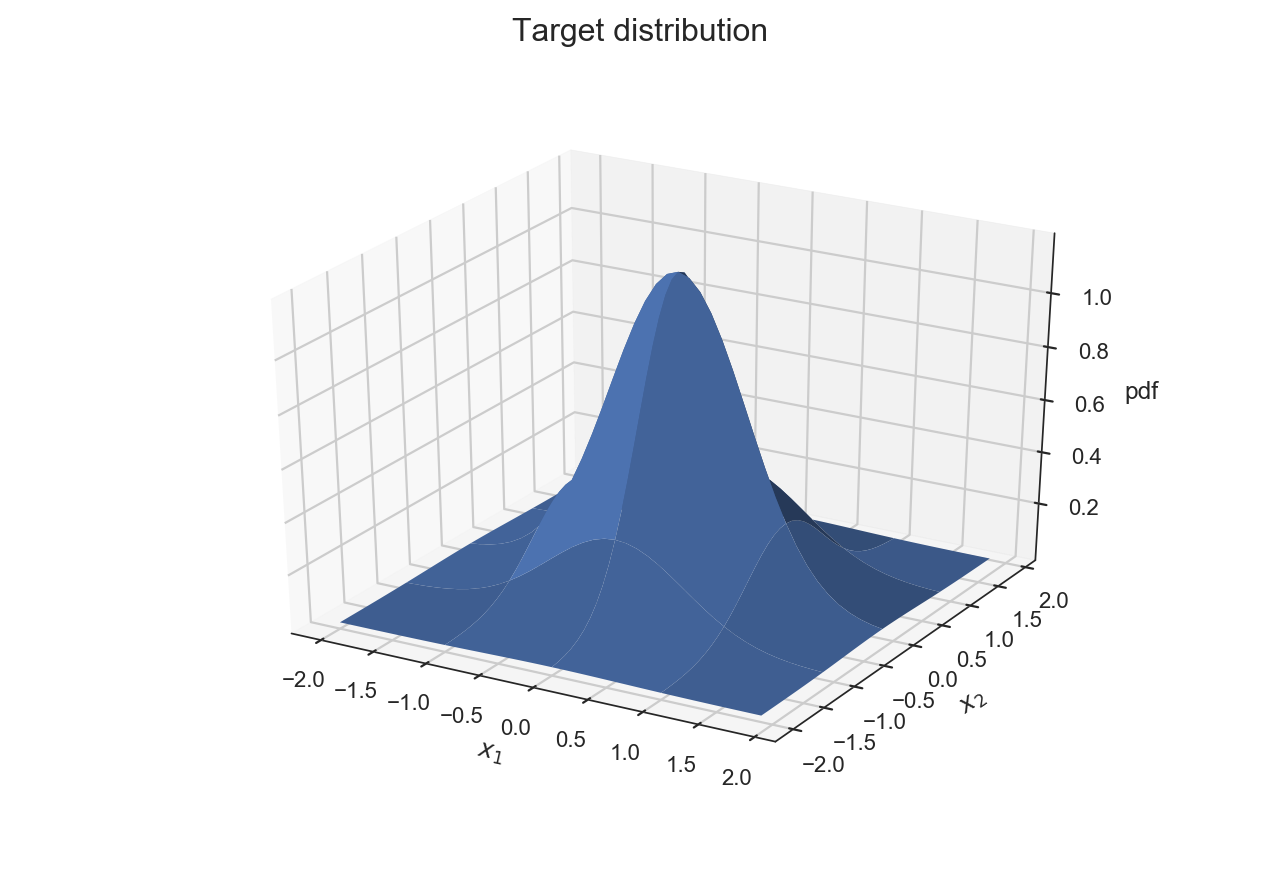
\includegraphics{../Figures/2.1.png}
		\caption{Target distribution for the MLP in the later exercises}
		\label{fig:2.1}
	\end{figure}
    \subsection{2}\label{section}
	The code provided below allows for plotting the progress over time. The naive output of the network is depicted in figure \ref{fig:2.2}.
	 

    \begin{Verbatim}[commandchars=\\\{\}]
{\color{incolor}In [{\color{incolor}97}]:} \PY{k}{class} \PY{n+nc}{mlp}\PY{p}{(}\PY{n+nb}{object}\PY{p}{)}\PY{p}{:}
             \PY{l+s+sd}{\PYZsq{}\PYZsq{}\PYZsq{}}
         \PY{l+s+sd}{    Multi\PYZhy{}layered\PYZhy{}pereptron}
         \PY{l+s+sd}{    K = output nodes}
         \PY{l+s+sd}{    M = hidden nodes}
         \PY{l+s+sd}{    Assumes the input data X is samples x feature dimension}
         \PY{l+s+sd}{    Returns:}
         \PY{l+s+sd}{        prediction and error}
         \PY{l+s+sd}{    \PYZsq{}\PYZsq{}\PYZsq{}}
             \PY{k}{def} \PY{n+nf}{\PYZus{}\PYZus{}init\PYZus{}\PYZus{}}\PY{p}{(}\PY{n+nb+bp}{self}\PY{p}{,} \PY{n}{X}\PY{p}{,} \PY{n}{t}\PY{p}{,}\PYZbs{}
                          \PY{n}{eta} \PY{o}{=} \PY{l+m+mi}{1}\PY{n}{e}\PY{o}{\PYZhy{}}\PY{l+m+mi}{1}\PY{p}{,}\PYZbs{}
                          \PY{n}{gamma} \PY{o}{=} \PY{o}{.}\PY{l+m+mi}{0}\PY{p}{,}\PYZbs{}
                          \PY{n}{M} \PY{o}{=} \PY{l+m+mi}{8}\PY{p}{,}\PYZbs{}
                          \PY{n}{K} \PY{o}{=} \PY{l+m+mi}{1}\PY{p}{)}\PY{p}{:}
                 \PY{c+c1}{\PYZsh{} learning rate / momentum rate}
                 \PY{n+nb+bp}{self}\PY{o}{.}\PY{n}{eta}        \PY{o}{=} \PY{n}{eta}
                 \PY{n+nb+bp}{self}\PY{o}{.}\PY{n}{gamma}      \PY{o}{=} \PY{n}{gamma}
                 \PY{c+c1}{\PYZsh{} Layer dimensions; input, hidden, output}
                 \PY{n+nb+bp}{self}\PY{o}{.}\PY{n}{D}          \PY{o}{=} \PY{n}{D} \PY{o}{=}  \PY{n}{X}\PY{o}{.}\PY{n}{shape}\PY{p}{[}\PY{l+m+mi}{1}\PY{p}{]} \PY{o}{+} \PY{l+m+mi}{1}
                 \PY{n+nb+bp}{self}\PY{o}{.}\PY{n}{M}          \PY{o}{=} \PY{n}{M}
                 \PY{n+nb+bp}{self}\PY{o}{.}\PY{n}{K}          \PY{o}{=} \PY{n}{K}
                 \PY{c+c1}{\PYZsh{} add bias node to input}
                 \PY{n+nb+bp}{self}\PY{o}{.}\PY{n}{X}          \PY{o}{=} \PY{n}{hstack}\PY{p}{(} \PY{p}{(}\PY{n}{X}\PY{p}{,} \PY{n}{ones}\PY{p}{(}\PY{p}{(} \PY{n}{X}\PY{o}{.}\PY{n}{shape}\PY{p}{[}\PY{l+m+mi}{0}\PY{p}{]}\PY{p}{,} \PY{l+m+mi}{1} \PY{p}{)} \PY{p}{)} \PY{p}{)} \PY{p}{)}
                 \PY{n+nb+bp}{self}\PY{o}{.}\PY{n}{targets}    \PY{o}{=} \PY{n}{t}
                 \PY{c+c1}{\PYZsh{} weights; hidden and output}
                 \PY{n}{wh}              \PY{o}{=} \PY{n}{random}\PY{o}{.}\PY{n}{rand}\PY{p}{(}\PY{n}{D}\PY{p}{,} \PY{n}{M}\PY{p}{)} \PY{o}{\PYZhy{}} \PY{l+m+mi}{1}\PY{o}{/}\PY{l+m+mi}{2}
                 \PY{n}{wo}              \PY{o}{=} \PY{n}{random}\PY{o}{.}\PY{n}{rand}\PY{p}{(}\PY{n}{M}\PY{p}{,} \PY{n}{K}\PY{p}{)} \PY{o}{\PYZhy{}} \PY{l+m+mi}{1}\PY{o}{/}\PY{l+m+mi}{2}
         
                 \PY{n+nb+bp}{self}\PY{o}{.}\PY{n}{layers}     \PY{o}{=} \PY{p}{[}\PY{n}{wh}\PY{p}{,} \PY{n}{wo}\PY{p}{]}
                 \PY{c+c1}{\PYZsh{} activation functions:}
                 \PY{n+nb+bp}{self}\PY{o}{.}\PY{n}{func}       \PY{o}{=} \PY{k}{lambda} \PY{n}{x}\PY{p}{:} \PY{n}{tanh}\PY{p}{(}\PY{n}{x}\PY{p}{)}
                 \PY{n+nb+bp}{self}\PY{o}{.}\PY{n}{dfunc}      \PY{o}{=} \PY{k}{lambda} \PY{n}{x}\PY{p}{:} \PY{l+m+mi}{1} \PY{o}{\PYZhy{}} \PY{n}{x}\PY{o}{*}\PY{o}{*}\PY{l+m+mi}{2}
                 
         
             \PY{k}{def} \PY{n+nf}{forwardSingle}\PY{p}{(}\PY{n+nb+bp}{self}\PY{p}{,} \PY{n}{xi}\PY{p}{)}\PY{p}{:}
                 \PY{l+s+sd}{\PYZsq{}\PYZsq{}\PYZsq{} Performs a single forward pass in the network\PYZsq{}\PYZsq{}\PYZsq{}}
                 \PY{n}{layerOutputs} \PY{o}{=} \PY{p}{[} \PY{p}{[}\PY{p}{]}  \PY{k}{for} \PY{n}{j} \PY{o+ow}{in} \PY{n+nb+bp}{self}\PY{o}{.}\PY{n}{layers} \PY{p}{]}
                 \PY{c+c1}{\PYZsh{}forward pass}
                 \PY{n}{a} \PY{o}{=} \PY{n}{xi}\PY{o}{.}\PY{n}{dot}\PY{p}{(}\PY{n+nb+bp}{self}\PY{o}{.}\PY{n}{layers}\PY{p}{[}\PY{l+m+mi}{0}\PY{p}{]}\PY{p}{)}
                 \PY{n}{z} \PY{o}{=} \PY{n+nb+bp}{self}\PY{o}{.}\PY{n}{func}\PY{p}{(}\PY{n}{a}\PY{p}{)}
                 \PY{n}{y} \PY{o}{=} \PY{n}{z}\PY{o}{.}\PY{n}{dot}\PY{p}{(}\PY{n+nb+bp}{self}\PY{o}{.}\PY{n}{layers}\PY{p}{[}\PY{l+m+mi}{1}\PY{p}{]}\PY{p}{)}
                 
                 \PY{c+c1}{\PYZsh{} save output}
                 \PY{n}{layerOutputs}\PY{p}{[}\PY{l+m+mi}{0}\PY{p}{]}\PY{o}{.}\PY{n}{append}\PY{p}{(}\PY{n}{z}\PY{p}{)}\PY{p}{;}
                 \PY{n}{layerOutputs}\PY{p}{[}\PY{l+m+mi}{1}\PY{p}{]}\PY{o}{.}\PY{n}{append}\PY{p}{(}\PY{n}{y}\PY{p}{)}
                 \PY{k}{return} \PY{n}{layerOutputs}
             
             \PY{k}{def} \PY{n+nf}{backwardsSingle}\PY{p}{(}\PY{n+nb+bp}{self}\PY{p}{,} \PY{n}{ti}\PY{p}{,} \PY{n}{xi}\PY{p}{,} \PY{n}{forwardPass}\PY{p}{)}\PY{p}{:}
                 \PY{l+s+sd}{\PYZsq{}\PYZsq{}\PYZsq{}Backprop + update of weights\PYZsq{}\PYZsq{}\PYZsq{}}
                 \PY{c+c1}{\PYZsh{} prediction error}
                 \PY{n}{dk} \PY{o}{=} \PY{n}{forwardPass}\PY{p}{[}\PY{o}{\PYZhy{}}\PY{l+m+mi}{1}\PY{p}{]}\PY{p}{[}\PY{l+m+mi}{0}\PY{p}{]} \PY{o}{\PYZhy{}} \PY{n}{ti}
                 \PY{n}{squaredError} \PY{o}{=} \PY{n}{dk}\PY{o}{*}\PY{o}{*}\PY{l+m+mi}{2}
                 \PY{c+c1}{\PYZsh{} compute hidden activation; note elementwise product!!}
                 \PY{n}{dj} \PY{o}{=} \PYZbs{}
                 \PY{n+nb+bp}{self}\PY{o}{.}\PY{n}{dfunc}\PY{p}{(}\PY{n}{forwardPass}\PY{p}{[}\PY{l+m+mi}{0}\PY{p}{]}\PY{p}{[}\PY{l+m+mi}{0}\PY{p}{]}\PY{p}{)} \PY{o}{*} \PY{p}{(}\PY{n}{dk}\PY{o}{.}\PY{n}{dot}\PY{p}{(}\PY{n+nb+bp}{self}\PY{o}{.}\PY{n}{layers}\PY{p}{[}\PY{o}{\PYZhy{}}\PY{l+m+mi}{1}\PY{p}{]}\PY{o}{.}\PY{n}{T}\PY{p}{)}\PY{p}{)}
         
                 \PY{c+c1}{\PYZsh{} update the weights}
                 \PY{n}{E1} \PY{o}{=} \PY{n}{forwardPass}\PY{p}{[}\PY{l+m+mi}{0}\PY{p}{]}\PY{p}{[}\PY{l+m+mi}{0}\PY{p}{]}\PY{o}{.}\PY{n}{T}\PY{o}{.}\PY{n}{dot}\PY{p}{(}\PY{n}{dk}\PY{p}{)}
                 \PY{n}{E2} \PY{o}{=} \PY{n}{xi}\PY{o}{.}\PY{n}{T}\PY{o}{.}\PY{n}{dot}\PY{p}{(}\PY{n}{dj}\PY{p}{)}
                 
                 \PY{c+c1}{\PYZsh{} update weights of layers}
                 \PY{n+nb+bp}{self}\PY{o}{.}\PY{n}{layers}\PY{p}{[}\PY{o}{\PYZhy{}}\PY{l+m+mi}{1}\PY{p}{]} \PY{o}{\PYZhy{}}\PY{o}{=} \PYZbs{}
                 \PY{n+nb+bp}{self}\PY{o}{.}\PY{n}{eta} \PY{o}{*} \PY{n}{E1} \PY{o}{+} \PY{n+nb+bp}{self}\PY{o}{.}\PY{n}{gamma} \PY{o}{*} \PY{n+nb+bp}{self}\PY{o}{.}\PY{n}{layers}\PY{p}{[}\PY{o}{\PYZhy{}}\PY{l+m+mi}{1}\PY{p}{]}
                 
                 \PY{n+nb+bp}{self}\PY{o}{.}\PY{n}{layers}\PY{p}{[}\PY{l+m+mi}{0}\PY{p}{]}  \PY{o}{\PYZhy{}}\PY{o}{=} \PYZbs{}
                 \PY{n+nb+bp}{self}\PY{o}{.}\PY{n}{eta} \PY{o}{*} \PY{n}{E2} \PY{o}{+} \PY{n+nb+bp}{self}\PY{o}{.}\PY{n}{gamma} \PY{o}{*} \PY{n+nb+bp}{self}\PY{o}{.}\PY{n}{layers}\PY{p}{[}\PY{l+m+mi}{0}\PY{p}{]}
                 \PY{k}{return} \PY{n}{squaredError}
             
             \PY{k}{def} \PY{n+nf}{train}\PY{p}{(}\PY{n+nb+bp}{self}\PY{p}{,} \PY{n}{num}\PY{p}{,} \PY{n}{plotProg} \PY{o}{=} \PY{p}{(}\PY{k+kc}{False}\PY{p}{,}\PY{p}{)}\PY{p}{)}\PY{p}{:}
                 \PY{c+c1}{\PYZsh{}set up figure}
                 \PY{k}{if} \PY{n}{plotProg}\PY{p}{[}\PY{l+m+mi}{0}\PY{p}{]}\PY{p}{:}
                     \PY{n}{fig}\PY{p}{,} \PY{n}{ax} \PY{o}{=} \PY{n}{subplots}\PY{p}{(}\PY{n}{subplot\PYZus{}kw} \PY{o}{=} \PY{p}{\PYZob{}}\PY{l+s+s1}{\PYZsq{}}\PY{l+s+s1}{projection}\PY{l+s+s1}{\PYZsq{}}\PY{p}{:}\PY{l+s+s1}{\PYZsq{}}\PY{l+s+s1}{3d}\PY{l+s+s1}{\PYZsq{}}\PY{p}{\PYZcb{}}\PY{p}{)}
         
                     
                 \PY{n}{num}   \PY{o}{=} \PY{n+nb}{int}\PY{p}{(}\PY{n}{num}\PY{p}{)} \PY{c+c1}{\PYZsh{} for scientific notation}
                 \PY{n}{SSE}   \PY{o}{=} \PY{n}{zeros}\PY{p}{(}\PY{n}{num}\PY{p}{)} \PY{c+c1}{\PYZsh{} sum squared error}
                 \PY{n}{preds} \PY{o}{=} \PY{n}{zeros}\PY{p}{(}\PY{p}{(}\PY{n}{num}\PY{p}{,} \PY{n+nb}{len}\PY{p}{(}\PY{n+nb+bp}{self}\PY{o}{.}\PY{n}{targets}\PY{p}{)}\PY{p}{)}\PY{p}{)} \PY{c+c1}{\PYZsh{} predictions per run}
                 \PY{k}{for} \PY{n+nb}{iter} \PY{o+ow}{in} \PY{n+nb}{range}\PY{p}{(}\PY{n}{num}\PY{p}{)}\PY{p}{:}
                     \PY{n}{error} \PY{o}{=} \PY{l+m+mi}{0} \PY{c+c1}{\PYZsh{} sum squared error}
                     \PY{k}{for} \PY{n}{idx}\PY{p}{,} \PY{p}{(}\PY{n}{ti}\PY{p}{,} \PY{n}{xi}\PY{p}{)} \PY{o+ow}{in} \PY{n+nb}{enumerate}\PY{p}{(}\PY{n+nb}{zip}\PY{p}{(}\PY{n+nb+bp}{self}\PY{o}{.}\PY{n}{targets}\PY{p}{,} \PY{n+nb+bp}{self}\PY{o}{.}\PY{n}{X}\PY{p}{)}\PY{p}{)}\PY{p}{:}
                         \PY{n}{xi} \PY{o}{=} \PY{n}{array}\PY{p}{(}\PY{n}{xi}\PY{p}{,} \PY{n}{ndmin} \PY{o}{=} \PY{l+m+mi}{2}\PY{p}{)}
         
                         \PY{n}{forwardPass} \PY{o}{=} \PY{n+nb+bp}{self}\PY{o}{.}\PY{n}{forwardSingle}\PY{p}{(}\PY{n}{xi}\PY{p}{)}
                         \PY{n}{error} \PY{o}{+}\PY{o}{=} \PY{n+nb+bp}{self}\PY{o}{.}\PY{n}{backwardsSingle}\PY{p}{(}\PY{n}{ti}\PY{p}{,} \PY{n}{xi}\PY{p}{,} \PY{n}{forwardPass}\PY{p}{)}
                         \PY{n}{preds}\PY{p}{[}\PY{n+nb}{iter}\PY{p}{,} \PY{n}{idx}\PY{p}{]} \PY{o}{=} \PY{n}{forwardPass}\PY{p}{[}\PY{o}{\PYZhy{}}\PY{l+m+mi}{1}\PY{p}{]}\PY{p}{[}\PY{l+m+mi}{0}\PY{p}{]}         
                     \PY{c+c1}{\PYZsh{} plot progress}
                     \PY{k}{if} \PY{n}{plotProg}\PY{p}{[}\PY{l+m+mi}{0}\PY{p}{]}\PY{p}{:}
                         \PY{k}{if} \PY{o+ow}{not} \PY{n+nb}{iter} \PY{o}{\PYZpc{}} \PY{n}{plotProg}\PY{p}{[}\PY{l+m+mi}{1}\PY{p}{]}\PY{p}{:}
                             \PY{n}{x}\PY{p}{,} \PY{n}{y} \PY{o}{=} \PY{n}{plotProg}\PY{p}{[}\PY{l+m+mi}{2}\PY{p}{]}
                             \PY{n}{ax}\PY{o}{.}\PY{n}{cla}\PY{p}{(}\PY{p}{)} \PY{c+c1}{\PYZsh{} ugly workaround }
                             \PY{n}{ax}\PY{o}{.}\PY{n}{plot\PYZus{}surface}\PY{p}{(}\PY{n}{x}\PY{p}{,} \PY{n}{y}\PY{p}{,} \PY{n}{preds}\PY{p}{[}\PY{n+nb}{iter}\PY{p}{,} \PY{p}{:}\PY{p}{]}\PY{o}{.}\PY{n}{reshape}\PY{p}{(}\PY{n}{x}\PY{o}{.}\PY{n}{shape}\PY{p}{)}\PY{p}{)}
                             \PY{n}{ax}\PY{o}{.}\PY{n}{set\PYZus{}xlabel}\PY{p}{(}\PY{l+s+s1}{\PYZsq{}}\PY{l+s+s1}{\PYZdl{}x\PYZus{}1\PYZdl{}}\PY{l+s+s1}{\PYZsq{}}\PY{p}{,} \PY{n}{labelpad} \PY{o}{=} \PY{l+m+mi}{20}\PY{p}{)}
                             \PY{n}{ax}\PY{o}{.}\PY{n}{set\PYZus{}ylabel}\PY{p}{(}\PY{l+s+s1}{\PYZsq{}}\PY{l+s+s1}{\PYZdl{}x\PYZus{}2\PYZdl{}}\PY{l+s+s1}{\PYZsq{}}\PY{p}{,} \PY{n}{labelpad} \PY{o}{=} \PY{l+m+mi}{20}\PY{p}{)}
                             \PY{n}{ax}\PY{o}{.}\PY{n}{set\PYZus{}zlabel}\PY{p}{(}\PY{l+s+s1}{\PYZsq{}}\PY{l+s+s1}{pdf}\PY{l+s+s1}{\PYZsq{}}\PY{p}{,} \PY{n}{labelpad} \PY{o}{=}\PY{l+m+mi}{20}\PY{p}{)}
                             \PY{n}{ax}\PY{o}{.}\PY{n}{set\PYZus{}title}\PY{p}{(}\PY{l+s+s1}{\PYZsq{}}\PY{l+s+s1}{Cycle = }\PY{l+s+si}{\PYZob{}0\PYZcb{}}\PY{l+s+s1}{\PYZsq{}}\PY{o}{.}\PY{n}{format}\PY{p}{(} \PY{n+nb}{iter} \PY{p}{)}\PY{p}{)}
                             \PY{n}{pause}\PY{p}{(}\PY{l+m+mi}{1}\PY{n}{e}\PY{o}{\PYZhy{}}\PY{l+m+mi}{10}\PY{p}{)}
                     \PY{n}{SSE}\PY{p}{[}\PY{n+nb}{iter}\PY{p}{]} \PY{o}{=} \PY{o}{.}\PY{l+m+mi}{5} \PY{o}{*} \PY{n}{error}
                 \PY{k}{return} \PY{n}{SSE}\PY{p}{,} \PY{n}{preds}
         
         \PY{c+c1}{\PYZsh{} perform a single forward pass and show the results}
         \PY{n}{model} \PY{o}{=} \PY{n}{mlp}\PY{p}{(}\PY{n}{X}\PY{p}{,} \PY{n}{targets}\PY{p}{)}
         \PY{c+c1}{\PYZsh{} perform a single pass}
         \PY{n}{preds} \PY{o}{=} \PY{n}{array}\PY{p}{(}\PY{p}{[}\PYZbs{}
                       \PY{n}{model}\PY{o}{.}\PY{n}{forwardSingle}\PY{p}{(}\PYZbs{}
                       \PY{n}{array}\PY{p}{(}\PY{n}{hstack}\PY{p}{(} \PY{p}{(} \PY{n}{xi}\PY{p}{,} \PY{l+m+mi}{1}\PY{p}{)} \PY{p}{)}\PY{p}{,}\PYZbs{}
                             \PY{n}{ndmin} \PY{o}{=} \PY{l+m+mi}{2}\PY{p}{)}\PY{p}{)}\PY{p}{[}\PY{o}{\PYZhy{}}\PY{l+m+mi}{1}\PY{p}{]}\PYZbs{}
                       \PY{k}{for} \PY{n}{xi} \PY{o+ow}{in} \PY{n}{X}\PY{p}{]}\PY{p}{)}\PY{o}{.}\PY{n}{flatten}\PY{p}{(}\PY{p}{)}
         \PY{c+c1}{\PYZsh{} plot the results}
         \PY{n}{fig}\PY{p}{,} \PY{n}{ax} \PY{o}{=} \PY{n}{subplots}\PY{p}{(}\PY{n}{subplot\PYZus{}kw}  \PY{o}{=} \PY{p}{\PYZob{}}\PY{l+s+s1}{\PYZsq{}}\PY{l+s+s1}{projection}\PY{l+s+s1}{\PYZsq{}}\PY{p}{:} \PY{l+s+s1}{\PYZsq{}}\PY{l+s+s1}{3d}\PY{l+s+s1}{\PYZsq{}}\PY{p}{\PYZcb{}}\PY{p}{)}
         \PY{n}{ax}\PY{o}{.}\PY{n}{scatter}\PY{p}{(}\PY{n}{x}\PY{p}{,} \PY{n}{y}\PY{p}{,} \PY{n}{preds}\PY{o}{.}\PY{n}{reshape}\PY{p}{(}\PY{n}{x}\PY{o}{.}\PY{n}{shape}\PY{p}{)}\PY{p}{)}
         \PY{n}{ax}\PY{o}{.}\PY{n}{set\PYZus{}xlabel}\PY{p}{(}\PY{l+s+s1}{\PYZsq{}}\PY{l+s+s1}{\PYZdl{}x\PYZus{}1\PYZdl{}}\PY{l+s+s1}{\PYZsq{}}\PY{p}{,} \PY{n}{labelpad} \PY{o}{=} \PY{l+m+mi}{20}\PY{p}{)}
         \PY{n}{ax}\PY{o}{.}\PY{n}{set\PYZus{}ylabel}\PY{p}{(}\PY{l+s+s1}{\PYZsq{}}\PY{l+s+s1}{\PYZdl{}x\PYZus{}2\PYZdl{}}\PY{l+s+s1}{\PYZsq{}}\PY{p}{,} \PY{n}{labelpad} \PY{o}{=} \PY{l+m+mi}{20}\PY{p}{)}
         \PY{n}{ax}\PY{o}{.}\PY{n}{set\PYZus{}zlabel}\PY{p}{(}\PY{l+s+s1}{\PYZsq{}}\PY{l+s+s1}{pdf}\PY{l+s+s1}{\PYZsq{}}\PY{p}{,} \PY{n}{labelpad} \PY{o}{=}\PY{l+m+mi}{20}\PY{p}{)}
         \PY{n}{ax}\PY{o}{.}\PY{n}{set\PYZus{}title}\PY{p}{(}\PY{l+s+s1}{\PYZsq{}}\PY{l+s+s1}{Network output without training}\PY{l+s+s1}{\PYZsq{}}\PY{p}{)}
         \PY{n}{sb}\PY{o}{.}\PY{n}{set\PYZus{}context}\PY{p}{(}\PY{l+s+s1}{\PYZsq{}}\PY{l+s+s1}{poster}\PY{l+s+s1}{\PYZsq{}}\PY{p}{)}
         \PY{n}{savefig}\PY{p}{(}\PY{l+s+s1}{\PYZsq{}}\PY{l+s+s1}{../Figures/2.2.png}\PY{l+s+s1}{\PYZsq{}}\PY{p}{)}
         \PY{n}{show}\PY{p}{(}\PY{p}{)}
\end{Verbatim}
	
	\begin{figure}[H]
		\centering 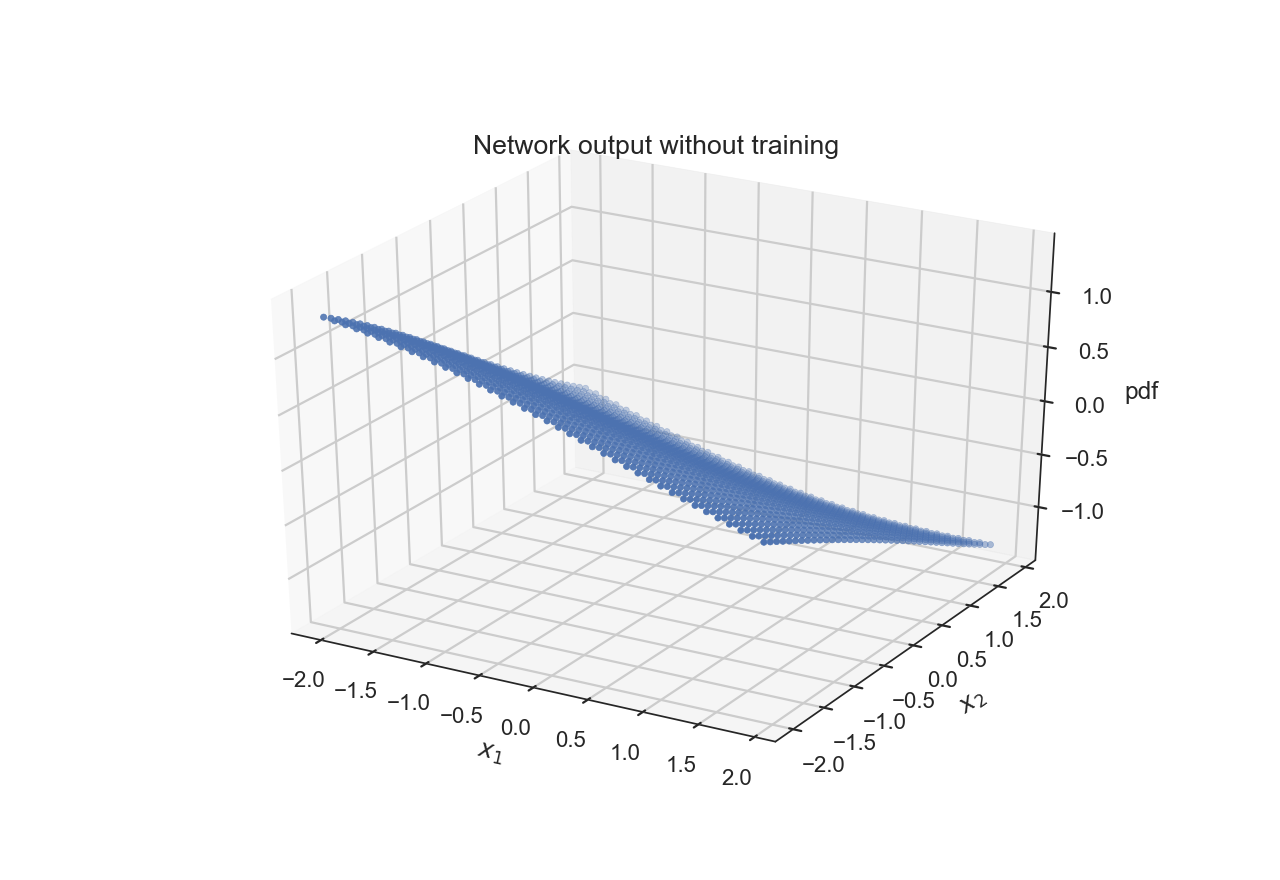
\includegraphics{../Figures/2.2.png}
		\caption{Results for 1.2; output of the network without any training.}
		\label{fig:1.2}
	\end{figure}

    \section{3}\label{section}
	If one wants to please parse the correct parameter, i.e. plotProg = (True, interval, [x,y]). As summary of the training progress is depicted in figure \ref{fig:2.3}. Please note that cylce = 0 is actually one fully completed training cycle as python starts indexing from 0. The zero training is shown in the previous question, i.e. figure \ref{fig:1.2}.
    \begin{Verbatim}[commandchars=\\\{\}]
{\color{incolor}In [{\color{incolor}98}]:} \PY{c+c1}{\PYZsh{} run at atleast 500 cycles}
         \PY{n}{num} \PY{o}{=} \PY{n+nb}{int}\PY{p}{(}\PY{l+m+mi}{5}\PY{n}{e2}\PY{p}{)} \PY{o}{+} \PY{l+m+mi}{1}
         \PY{n}{model} \PY{o}{=} \PY{n}{mlp}\PY{p}{(}\PY{n}{X}\PY{p}{,} \PY{n}{targets}\PY{p}{)}
         \PY{c+c1}{\PYZsh{} train the model}
         \PY{n}{SSE}\PY{p}{,} \PY{n}{preds} \PY{o}{=} \PY{n}{model}\PY{o}{.}\PY{n}{train}\PY{p}{(}\PY{n}{num}\PY{p}{)}
\end{Verbatim}

    \begin{Verbatim}[commandchars=\\\{\}]
{\color{incolor}In [{\color{incolor}82}]:} \PY{c+c1}{\PYZsh{} plot every 250 cycles}
         \PY{n}{cycleRange} \PY{o}{=} \PY{n}{arange}\PY{p}{(}\PY{l+m+mi}{0}\PY{p}{,}  \PY{n}{num}\PY{p}{,} \PY{n}{num} \PY{o}{/}\PY{o}{/} \PY{l+m+mi}{5}\PY{p}{)}
         
         \PY{c+c1}{\PYZsh{} use at most 3 rows}
         \PY{n}{nRows} \PY{o}{=} \PY{l+m+mi}{3}
         \PY{n}{nCols} \PY{o}{=} \PY{n+nb}{int}\PY{p}{(}\PY{n}{ceil}\PY{p}{(}\PY{n+nb}{len}\PY{p}{(}\PY{n}{cycleRange}\PY{p}{)}\PY{o}{/}\PY{n}{nRows}\PY{p}{)}\PY{p}{)}
         \PY{n}{nCols} \PY{o}{=} \PY{l+m+mi}{2}
         
         \PY{n}{fig}\PY{p}{,} \PY{n}{axes}  \PY{o}{=} \PY{n}{subplots}\PY{p}{(}\PY{n}{nRows}\PY{p}{,}\PYZbs{}
                               \PY{n}{nCols}\PY{p}{,}\PYZbs{}
                               \PY{n}{subplot\PYZus{}kw} \PY{o}{=} \PY{p}{\PYZob{}}\PY{l+s+s1}{\PYZsq{}}\PY{l+s+s1}{projection}\PY{l+s+s1}{\PYZsq{}}\PY{p}{:} \PY{l+s+s1}{\PYZsq{}}\PY{l+s+s1}{3d}\PY{l+s+s1}{\PYZsq{}}\PY{p}{\PYZcb{}}\PY{p}{)}
         
         
         \PY{k}{for} \PY{n}{axi}\PY{p}{,} \PY{n}{i} \PY{o+ow}{in} \PY{n+nb}{enumerate}\PY{p}{(}\PY{n}{cycleRange}\PY{p}{)}\PY{p}{:}
             \PY{n}{ax} \PY{o}{=} \PY{n}{axes}\PY{o}{.}\PY{n}{flatten}\PY{p}{(}\PY{p}{)}\PY{p}{[}\PY{n}{axi}\PY{p}{]}
             \PY{n}{ax}\PY{o}{.}\PY{n}{plot\PYZus{}surface}\PY{p}{(}\PYZbs{}
                             \PY{n}{x}\PY{p}{,}\PYZbs{}
                             \PY{n}{y}\PY{p}{,}\PYZbs{}
                             \PY{n}{preds}\PY{p}{[}\PY{n}{i}\PY{p}{,}\PY{p}{:}\PY{p}{]}\PY{o}{.}\PY{n}{reshape}\PY{p}{(}\PY{n}{x}\PY{o}{.}\PY{n}{shape}\PY{p}{)}\PY{p}{,}\PYZbs{}
                             \PY{n}{cstride} \PY{o}{=} \PY{l+m+mi}{1}\PY{p}{,}\PYZbs{}
                             \PY{n}{rstride} \PY{o}{=} \PY{l+m+mi}{1}\PY{p}{)}
             \PY{c+c1}{\PYZsh{} formatting of plot}
             \PY{n}{ax}\PY{o}{.}\PY{n}{set\PYZus{}xlabel}\PY{p}{(}\PY{l+s+s1}{\PYZsq{}}\PY{l+s+s1}{\PYZdl{}x\PYZus{}1\PYZdl{}}\PY{l+s+s1}{\PYZsq{}}\PY{p}{,} \PY{n}{labelpad} \PY{o}{=} \PY{l+m+mi}{20}\PY{p}{)}
             \PY{n}{ax}\PY{o}{.}\PY{n}{set\PYZus{}ylabel}\PY{p}{(}\PY{l+s+s1}{\PYZsq{}}\PY{l+s+s1}{\PYZdl{}x\PYZus{}2\PYZdl{}}\PY{l+s+s1}{\PYZsq{}}\PY{p}{,} \PY{n}{labelpad} \PY{o}{=} \PY{l+m+mi}{20}\PY{p}{)}
             \PY{n}{ax}\PY{o}{.}\PY{n}{set\PYZus{}zlabel}\PY{p}{(}\PY{l+s+s1}{\PYZsq{}}\PY{l+s+s1}{pdf}\PY{l+s+s1}{\PYZsq{}}\PY{p}{,} \PY{n}{labelpad} \PY{o}{=}\PY{l+m+mi}{20}\PY{p}{)}
             \PY{n}{ax}\PY{o}{.}\PY{n}{set\PYZus{}title}\PY{p}{(}\PY{l+s+s1}{\PYZsq{}}\PY{l+s+s1}{cycles = }\PY{l+s+si}{\PYZob{}0\PYZcb{}}\PY{l+s+s1}{\PYZsq{}}\PY{o}{.}\PY{n}{format}\PY{p}{(}\PY{n}{i}\PY{p}{)}\PY{p}{)}
             \PY{n}{sb}\PY{o}{.}\PY{n}{set\PYZus{}style}\PY{p}{(}\PY{l+s+s1}{\PYZsq{}}\PY{l+s+s1}{white}\PY{l+s+s1}{\PYZsq{}}\PY{p}{)}
         \PY{n}{fig}\PY{o}{.}\PY{n}{delaxes}\PY{p}{(}\PY{n}{axes}\PY{o}{.}\PY{n}{flatten}\PY{p}{(}\PY{p}{)}\PY{p}{[}\PY{o}{\PYZhy{}}\PY{l+m+mi}{1}\PY{p}{]}\PY{p}{)}
         \PY{n}{fig}\PY{o}{.}\PY{n}{suptitle}\PY{p}{(}\PY{l+s+s1}{\PYZsq{}}\PY{l+s+s1}{Output of MLP as a function of complete cycles}\PY{l+s+s1}{\PYZsq{}}\PY{p}{)}
         \PY{n}{subplots\PYZus{}adjust}\PY{p}{(}\PY{n}{top}\PY{o}{=}\PY{l+m+mf}{0.8}\PY{p}{)}
         \PY{c+c1}{\PYZsh{} fig.tight\PYZus{}layout()}
         \PY{n}{savefig}\PY{p}{(}\PY{l+s+s1}{\PYZsq{}}\PY{l+s+s1}{../Figures/2.3.png}\PY{l+s+s1}{\PYZsq{}}\PY{p}{)}
         \PY{n}{show}\PY{p}{(}\PY{p}{)}
\end{Verbatim}
	\begin{figure}[H]
		\centering 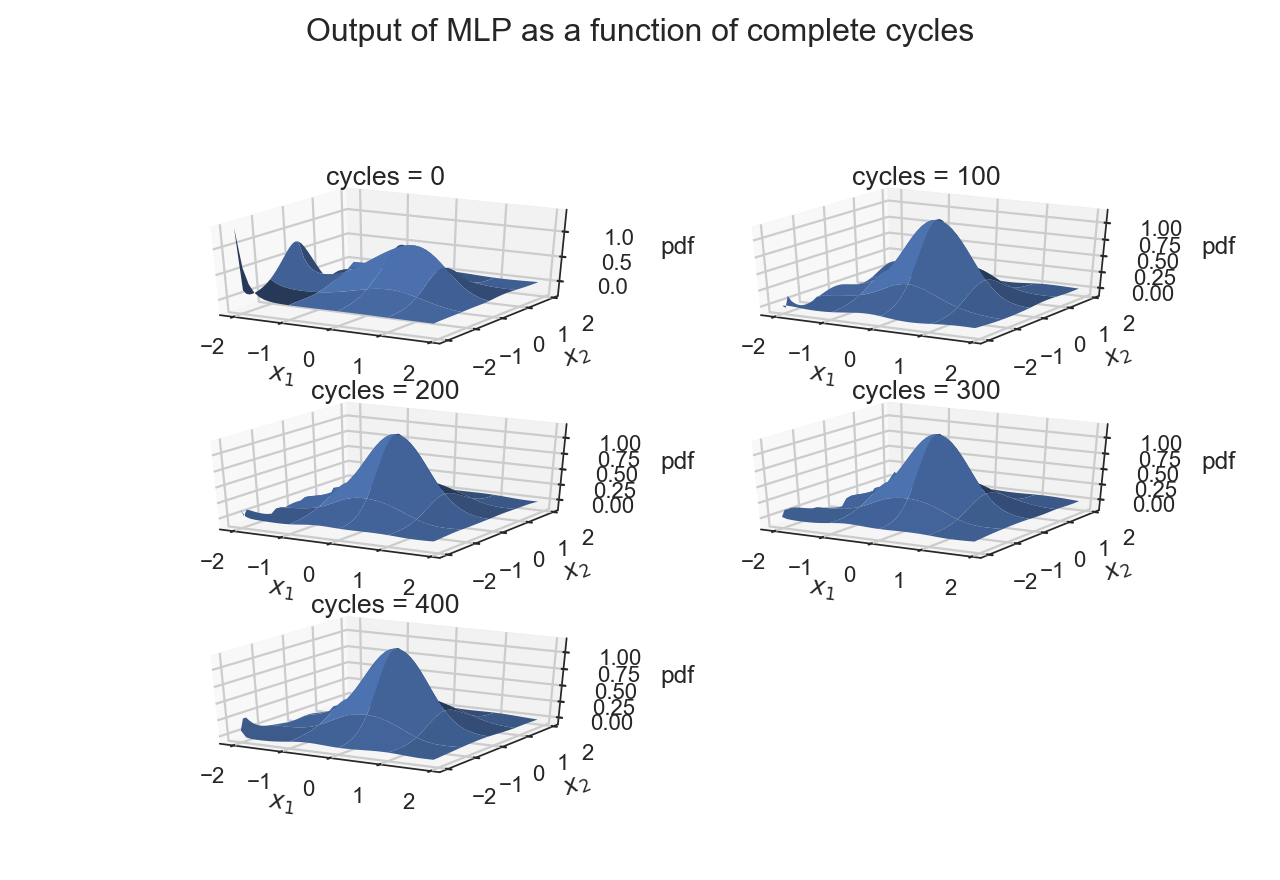
\includegraphics{../Figures/2.3.png}
		\caption{This figure shows the output of the network as a function of training cycles. Note that cycle = 0 is after 1 full pass of the network. Python starts indexing from 0. This if for the non-shuffled data.}
		\label{fig:2.3}
	\end{figure}
    \section{4}\label{section}
	Permute the indices and plot the sum squared error for the training. We expect the shuffled condition to have faster convergence. Results are shown in figure \ref{fig:2.4}.
    \begin{Verbatim}[commandchars=\\\{\}]
{\color{incolor}In [{\color{incolor}87}]:} \PY{c+c1}{\PYZsh{} shuffle the indices}
         \PY{n}{idx} \PY{o}{=} \PY{n}{random}\PY{o}{.}\PY{n}{permutation}\PY{p}{(}\PY{n+nb}{len}\PY{p}{(}\PY{n}{targets}\PY{p}{)}\PY{p}{)}
         
         \PY{c+c1}{\PYZsh{} shuffle the data}
         \PY{n}{shuffleX} \PY{o}{=} \PY{n}{X}\PY{p}{[}\PY{n}{idx}\PY{p}{,}\PY{p}{:}\PY{p}{]}
         \PY{c+c1}{\PYZsh{} shuffle the targets as well (same indices)}
         \PY{n}{shuffleTargets} \PY{o}{=} \PY{n}{targets}\PY{p}{[}\PY{n}{idx}\PY{p}{,} \PY{p}{:}\PY{p}{]}
         \PY{n}{shuffleModel} \PY{o}{=} \PY{n}{mlp}\PY{p}{(}\PY{n}{shuffleX}\PY{p}{,} \PY{n}{shuffleTargets}\PY{p}{)}
         \PY{n}{shuffleSSE}\PY{p}{,} \PY{n}{shufflePreds} \PY{o}{=} \PY{n}{shuffleModel}\PY{o}{.}\PY{n}{train}\PY{p}{(}\PY{n}{num}\PY{p}{)}
\end{Verbatim}

    \begin{Verbatim}[commandchars=\\\{\}]
{\color{incolor}In [{\color{incolor}90}]:} \PY{c+c1}{\PYZsh{} plot the results: compare with error from [3]}
         \PY{n}{fig}\PY{p}{,} \PY{n}{ax} \PY{o}{=} \PY{n}{subplots}\PY{p}{(}\PY{p}{)}
         \PY{n}{ax}\PY{o}{.}\PY{n}{plot}\PY{p}{(} \PY{n+nb}{range}\PY{p}{(}\PY{n}{num}\PY{p}{)}\PY{p}{,}\PY{n}{SSE}\PY{p}{,}\PYZbs{}
                 \PY{n+nb}{range}\PY{p}{(}\PY{n}{num}\PY{p}{)}\PY{p}{,} \PY{n}{shuffleSSE}\PY{p}{)}
         
         \PY{n}{ax}\PY{o}{.}\PY{n}{set\PYZus{}xlabel}\PY{p}{(}\PY{l+s+s1}{\PYZsq{}}\PY{l+s+s1}{Iterations}\PY{l+s+s1}{\PYZsq{}}\PY{p}{)}
         \PY{n}{ax}\PY{o}{.}\PY{n}{set\PYZus{}ylabel}\PY{p}{(}\PY{l+s+s1}{\PYZsq{}}\PY{l+s+s1}{Sum squared error}\PY{l+s+s1}{\PYZsq{}}\PY{p}{)}
         \PY{n}{ax}\PY{o}{.}\PY{n}{legend}\PY{p}{(}\PY{p}{[}\PY{l+s+s1}{\PYZsq{}}\PY{l+s+s1}{shuffled}\PY{l+s+s1}{\PYZsq{}}\PY{p}{,}\PY{l+s+s1}{\PYZsq{}}\PY{l+s+s1}{non\PYZhy{}shuffled}\PY{l+s+s1}{\PYZsq{}}\PY{p}{]}\PY{p}{,}\PY{n}{loc} \PY{o}{=} \PY{l+m+mi}{0}\PY{p}{)}
         \PY{n}{fig}\PY{o}{.}\PY{n}{suptitle}\PY{p}{(}\PY{l+s+s1}{\PYZsq{}}\PY{l+s+s1}{Training error}\PY{l+s+s1}{\PYZsq{}}\PY{p}{)}
         \PY{n}{savefig}\PY{p}{(}\PY{l+s+s1}{\PYZsq{}}\PY{l+s+s1}{../Figures/2.4.png}\PY{l+s+s1}{\PYZsq{}}\PY{p}{)}
         \PY{n}{show}\PY{p}{(}\PY{p}{)}
\end{Verbatim}
	\begin{figure}[H]
	\centering 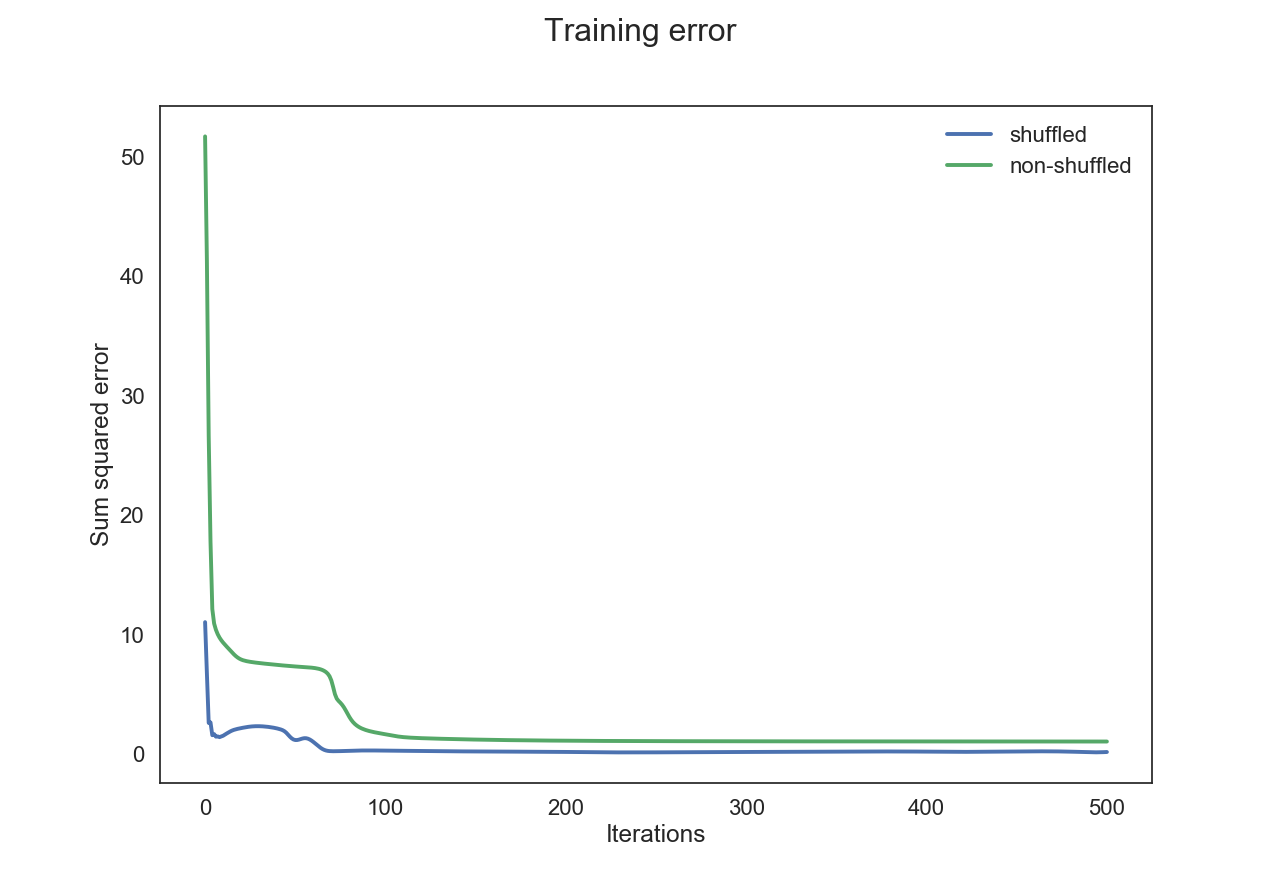
\includegraphics{../Figures/2.4}
	\caption{The sum squared error as a function of training cycles. Note a full cycle is after seeing all the training samples, weights are updated after seeing a datapoint. Noticeably, we see that the shuffled data is faster in converging, for explanation see text.}
	\label{fig:2.4}
\end{figure}
    Since the grid is linearly spaced, this will mean that nearby points
will yield the same gradient in the error. This `local' correlation will
yield that the algorithm will change the weights in similar direction
for a while, hence shuffling the data removes this `local' correlation
structure, yielding more likely to move in the different directions,
constraining the algorithm, yielding faster convergence.

    \section{5}\label{section}
	Same as in section 1.
	The target distribution is shown in figure \ref{fig:2.5}. 
	
    \begin{Verbatim}[commandchars=\\\{\}]
{\color{incolor}In [{\color{incolor}99}]:} \PY{c+c1}{\PYZsh{} load the data}
         \PY{n}{X}\PY{p}{,} \PY{n}{Y}\PY{p}{,} \PY{n}{target} \PY{o}{=} \PY{n+nb}{list}\PY{p}{(}\PY{n}{np}\PY{o}{.}\PY{n}{loadtxt}\PY{p}{(}\PY{l+s+s1}{\PYZsq{}}\PY{l+s+s1}{../Data/a017\PYZus{}NNpdfGaussMix.txt}\PY{l+s+s1}{\PYZsq{}}\PY{p}{)}\PY{o}{.}\PY{n}{T}\PY{p}{)}
         \PY{n}{tmp} \PY{o}{=} \PY{n+nb}{int}\PY{p}{(}\PY{n}{np}\PY{o}{.}\PY{n}{sqrt}\PY{p}{(}\PY{n}{target}\PY{o}{.}\PY{n}{shape}\PY{p}{[}\PY{l+m+mi}{0}\PY{p}{]}\PY{p}{)}\PY{p}{)}
         \PY{c+c1}{\PYZsh{} convert in shape for it to be plottable }
         \PY{n}{x} \PY{o}{=} \PY{n}{X}\PY{o}{.}\PY{n}{reshape}\PY{p}{(}\PY{n}{tmp}\PY{p}{,}\PY{n}{tmp}\PY{p}{)}
         
         \PY{n}{y} \PY{o}{=} \PY{n}{Y}\PY{o}{.}\PY{n}{reshape}\PY{p}{(}\PY{n}{tmp}\PY{p}{,} \PY{n}{tmp}\PY{p}{)}
         \PY{c+c1}{\PYZsh{} stack to create input data}
         \PY{n}{X} \PY{o}{=} \PY{n}{np}\PY{o}{.}\PY{n}{vstack}\PY{p}{(}\PY{p}{(}\PY{n}{X}\PY{p}{,}\PY{n}{Y}\PY{p}{)}\PY{p}{)}\PY{o}{.}\PY{n}{T}
         
         \PY{c+c1}{\PYZsh{} target vector}
         \PY{n}{target} \PY{o}{=} \PY{n}{np}\PY{o}{.}\PY{n}{array}\PY{p}{(}\PY{n}{target}\PY{p}{,} \PY{n}{ndmin} \PY{o}{=} \PY{l+m+mi}{2}\PY{p}{)}\PY{o}{.}\PY{n}{T}
\end{Verbatim}

    \begin{Verbatim}[commandchars=\\\{\}]
{\color{incolor}In [{\color{incolor}92}]:} \PY{c+c1}{\PYZsh{} visualize the target distribution}
         \PY{n}{fig}\PY{p}{,} \PY{n}{ax} \PY{o}{=} \PY{n}{subplots}\PY{p}{(}\PY{l+m+mi}{1}\PY{p}{,}\PY{l+m+mi}{1}\PY{p}{,} \PY{n}{subplot\PYZus{}kw} \PY{o}{=} \PY{p}{\PYZob{}}\PY{l+s+s1}{\PYZsq{}}\PY{l+s+s1}{projection}\PY{l+s+s1}{\PYZsq{}}\PY{p}{:} \PY{l+s+s1}{\PYZsq{}}\PY{l+s+s1}{3d}\PY{l+s+s1}{\PYZsq{}}\PY{p}{\PYZcb{}}\PY{p}{)}
         \PY{n}{ax}\PY{o}{.}\PY{n}{plot\PYZus{}surface}\PY{p}{(}\PY{n}{x}\PY{p}{,} \PY{n}{y}\PY{p}{,} \PY{n}{target}\PY{o}{.}\PY{n}{reshape}\PY{p}{(}\PY{n}{tmp}\PY{p}{,} \PY{n}{tmp}\PY{p}{)}\PY{p}{)}
         \PY{n}{ax}\PY{o}{.}\PY{n}{set\PYZus{}xlabel}\PY{p}{(}\PY{l+s+s1}{\PYZsq{}}\PY{l+s+s1}{\PYZdl{}x\PYZus{}1\PYZdl{}}\PY{l+s+s1}{\PYZsq{}}\PY{p}{,} \PY{n}{labelpad} \PY{o}{=} \PY{l+m+mi}{20}\PY{p}{)}
         \PY{n}{ax}\PY{o}{.}\PY{n}{set\PYZus{}ylabel}\PY{p}{(}\PY{l+s+s1}{\PYZsq{}}\PY{l+s+s1}{\PYZdl{}x\PYZus{}2\PYZdl{}}\PY{l+s+s1}{\PYZsq{}}\PY{p}{,} \PY{n}{labelpad} \PY{o}{=} \PY{l+m+mi}{20}\PY{p}{)}
         \PY{n}{ax}\PY{o}{.}\PY{n}{set\PYZus{}zlabel}\PY{p}{(}\PY{l+s+s1}{\PYZsq{}}\PY{l+s+s1}{pdf}\PY{l+s+s1}{\PYZsq{}}\PY{p}{,} \PY{n}{labelpad} \PY{o}{=} \PY{l+m+mi}{20}\PY{p}{)}
         \PY{n}{fig}\PY{o}{.}\PY{n}{suptitle}\PY{p}{(}\PY{l+s+s1}{\PYZsq{}}\PY{l+s+s1}{Target distribution}\PY{l+s+s1}{\PYZsq{}}\PY{p}{)}
         \PY{n}{savefig}\PY{p}{(}\PY{l+s+s1}{\PYZsq{}}\PY{l+s+s1}{../Figures/2.5.png}\PY{l+s+s1}{\PYZsq{}}\PY{p}{)}
         \PY{n}{show}\PY{p}{(}\PY{p}{)}
\end{Verbatim}

	\begin{figure}[H]
		\centering 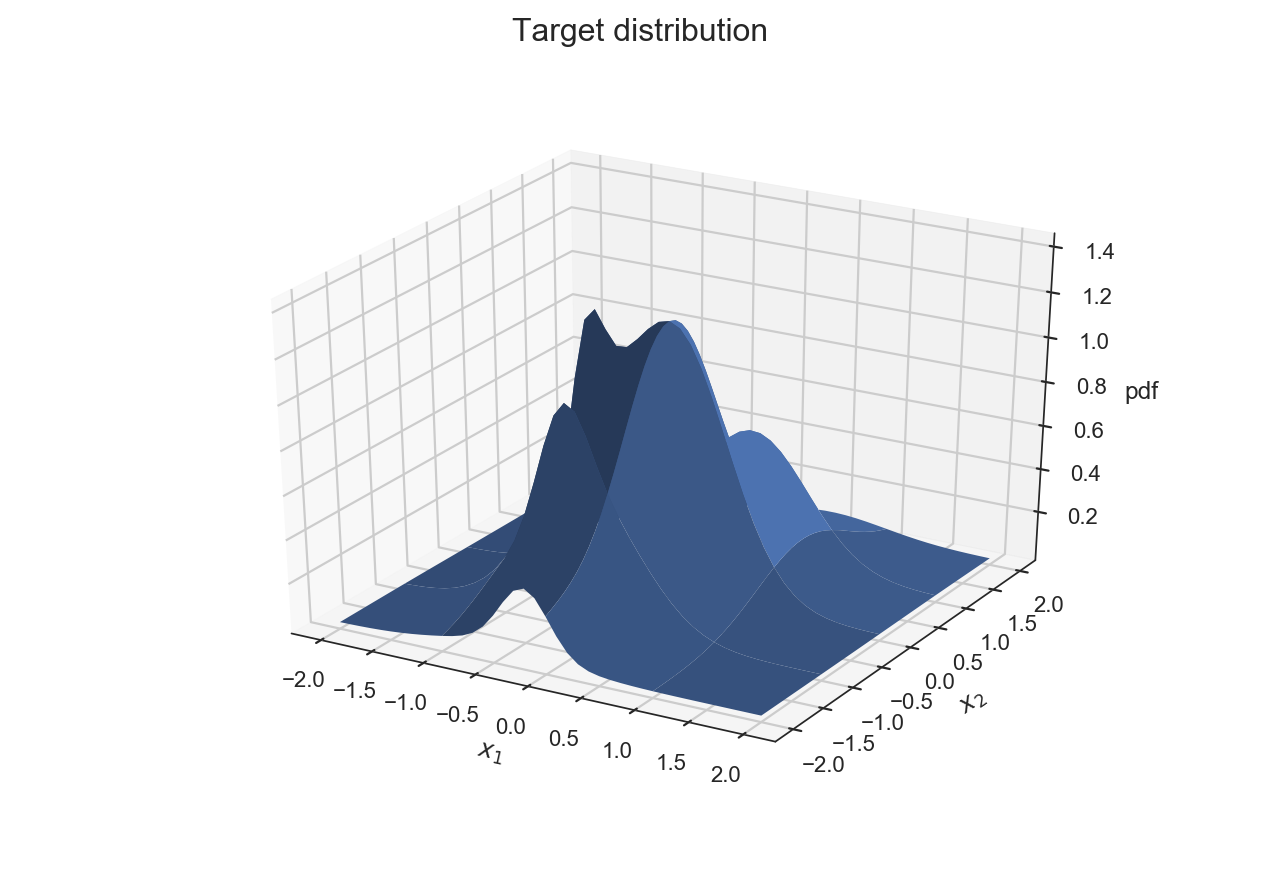
\includegraphics{../Figures/2.5.png}
		\caption{Target distribution loaded from the provided data files}
		\label{fig:2.5}
	\end{figure}

    \section{6}\label{section}
	The training error and final prediction are shown in figures \ref{fig:2.62}, \ref{fig:2.61}.
	Explanation is below the code block.
    \begin{Verbatim}[commandchars=\\\{\}]
{\color{incolor}In [{\color{incolor}100}]:} \PY{c+c1}{\PYZsh{}randomly permute indices}
          \PY{n}{idx} \PY{o}{=} \PY{n}{np}\PY{o}{.}\PY{n}{random}\PY{o}{.}\PY{n}{permutation}\PY{p}{(}\PY{n+nb}{range}\PY{p}{(}\PY{n+nb}{len}\PY{p}{(}\PY{n}{target}\PY{p}{)}\PY{p}{)}\PY{p}{)}
          \PY{c+c1}{\PYZsh{} keep track of the changes}
          \PY{n}{shuffX} \PY{o}{=} \PY{n}{X}\PY{p}{[}\PY{n}{idx}\PY{p}{,}\PY{p}{:}\PY{p}{]}\PY{p}{;} \PY{n}{shuffTarget} \PY{o}{=} \PY{n}{target}\PY{p}{[}\PY{n}{idx}\PY{p}{]}
          \PY{c+c1}{\PYZsh{} run mlp with eta = .01}
          \PY{n}{model} \PY{o}{=} \PY{n}{mlp}\PY{p}{(}\PY{n}{shuffX}\PY{p}{,} \PY{n}{shuffTarget}\PY{p}{,}\PYZbs{}
                              \PY{n}{eta} \PY{o}{=} \PY{l+m+mi}{1}\PY{n}{e}\PY{o}{\PYZhy{}}\PY{l+m+mi}{2}\PY{p}{,}\PYZbs{}
                              \PY{n}{M} \PY{o}{=} \PY{l+m+mi}{40}\PY{p}{)}
          
          \PY{c+c1}{\PYZsh{} run for 2000 complete cylcles}
          \PY{n}{num} \PY{o}{=} \PY{n+nb}{int}\PY{p}{(}\PY{l+m+mi}{2}\PY{n}{e3}\PY{p}{)}
          \PY{n}{errors}\PY{p}{,} \PY{n}{preds} \PY{o}{=} \PY{n}{model}\PY{o}{.}\PY{n}{train}\PY{p}{(}\PY{n}{num} \PY{o}{=} \PY{n}{num}\PY{p}{)}
          \PY{c+c1}{\PYZsh{} map back to original space}
          \PY{n}{orgIdx} \PY{o}{=} \PY{n}{argsort}\PY{p}{(}\PY{n}{idx}\PY{p}{)}
          \PY{c+c1}{\PYZsh{} get final prediction}
          \PY{n}{finalPred} \PY{o}{=} \PY{n}{preds}\PY{p}{[}\PY{o}{\PYZhy{}}\PY{l+m+mi}{1}\PY{p}{,} \PY{n}{orgIdx}\PY{p}{]}
\end{Verbatim}
	
    \begin{Verbatim}[commandchars=\\\{\}]
{\color{incolor}In [{\color{incolor}94}]:} \PY{c+c1}{\PYZsh{} plot the final prediction and the target distribution}
         \PY{n}{fig}\PY{p}{,} \PY{n}{ax} \PY{o}{=} \PY{n}{subplots}\PY{p}{(}\PY{n}{subplot\PYZus{}kw} \PY{o}{=} \PY{p}{\PYZob{}}\PY{l+s+s1}{\PYZsq{}}\PY{l+s+s1}{projection}\PY{l+s+s1}{\PYZsq{}}\PY{p}{:} \PY{l+s+s1}{\PYZsq{}}\PY{l+s+s1}{3d}\PY{l+s+s1}{\PYZsq{}}\PY{p}{\PYZcb{}}\PY{p}{)}
         \PY{n}{ax}\PY{o}{.}\PY{n}{scatter}\PY{p}{(}\PY{n}{x}\PY{p}{,} \PY{n}{y}\PY{p}{,} \PY{n}{target}\PY{o}{.}\PY{n}{reshape}\PY{p}{(}\PY{n}{x}\PY{o}{.}\PY{n}{shape}\PY{p}{)}\PY{p}{,} \PY{n}{label} \PY{o}{=} \PY{l+s+s1}{\PYZsq{}}\PY{l+s+s1}{target}\PY{l+s+s1}{\PYZsq{}}\PY{p}{)}
         \PY{n}{ax}\PY{o}{.}\PY{n}{scatter}\PY{p}{(}\PY{n}{x}\PY{p}{,} \PY{n}{y}\PY{p}{,} \PY{n}{finalPred}\PY{o}{.}\PY{n}{reshape}\PY{p}{(}\PY{n}{x}\PY{o}{.}\PY{n}{shape}\PY{p}{)}\PY{p}{,} \PY{n}{label} \PY{o}{=} \PY{l+s+s1}{\PYZsq{}}\PY{l+s+s1}{estimation}\PY{l+s+s1}{\PYZsq{}}\PY{p}{)}
         \PY{n}{ax}\PY{o}{.}\PY{n}{set\PYZus{}xlabel}\PY{p}{(}\PY{l+s+s1}{\PYZsq{}}\PY{l+s+s1}{\PYZdl{}x\PYZus{}1\PYZdl{}}\PY{l+s+s1}{\PYZsq{}}\PY{p}{,} \PY{n}{labelpad} \PY{o}{=} \PY{l+m+mi}{20}\PY{p}{)}
         \PY{n}{ax}\PY{o}{.}\PY{n}{set\PYZus{}ylabel}\PY{p}{(}\PY{l+s+s1}{\PYZsq{}}\PY{l+s+s1}{\PYZdl{}x\PYZus{}2\PYZdl{}}\PY{l+s+s1}{\PYZsq{}}\PY{p}{,} \PY{n}{labelpad} \PY{o}{=} \PY{l+m+mi}{20}\PY{p}{)}
         \PY{n}{ax}\PY{o}{.}\PY{n}{set\PYZus{}zlabel}\PY{p}{(}\PY{l+s+s1}{\PYZsq{}}\PY{l+s+s1}{pdf}\PY{l+s+s1}{\PYZsq{}}\PY{p}{,} \PY{n}{labelpad}   \PY{o}{=} \PY{l+m+mi}{20}\PY{p}{)}
         \PY{n}{ax}\PY{o}{.}\PY{n}{legend}\PY{p}{(}\PY{n}{loc} \PY{o}{=} \PY{l+m+mi}{0}\PY{p}{)}
         \PY{n}{fig}\PY{o}{.}\PY{n}{suptitle}\PY{p}{(}\PY{l+s+s1}{\PYZsq{}}\PY{l+s+s1}{Final prediction after }\PY{l+s+si}{\PYZob{}0\PYZcb{}}\PY{l+s+s1}{ cycles}\PY{l+s+s1}{\PYZsq{}}\PY{o}{.}\PY{n}{format}\PY{p}{(}\PY{n}{num}\PY{p}{)}\PY{p}{)}
         \PY{n}{savefig}\PY{p}{(}\PY{l+s+s1}{\PYZsq{}}\PY{l+s+s1}{../Figures/2.61.png}\PY{l+s+s1}{\PYZsq{}}\PY{p}{)}
         
         \PY{n}{fig}\PY{p}{,} \PY{n}{ax} \PY{o}{=} \PY{n}{subplots}\PY{p}{(}\PY{p}{)}
         \PY{n}{ax}\PY{o}{.}\PY{n}{plot}\PY{p}{(}\PY{n}{errors}\PY{p}{)}
         \PY{n}{ax}\PY{o}{.}\PY{n}{set\PYZus{}xlabel}\PY{p}{(}\PY{l+s+s1}{\PYZsq{}}\PY{l+s+s1}{iterations}\PY{l+s+s1}{\PYZsq{}}\PY{p}{)}
         \PY{n}{ax}\PY{o}{.}\PY{n}{set\PYZus{}ylabel}\PY{p}{(}\PY{l+s+s1}{\PYZsq{}}\PY{l+s+s1}{Sum squared error}\PY{l+s+s1}{\PYZsq{}}\PY{p}{)}
         \PY{n}{ax}\PY{o}{.}\PY{n}{set\PYZus{}title}\PY{p}{(}\PY{l+s+s1}{\PYZsq{}}\PY{l+s+s1}{Training error}\PY{l+s+s1}{\PYZsq{}}\PY{p}{)}
         \PY{n}{savefig}\PY{p}{(}\PY{l+s+s1}{\PYZsq{}}\PY{l+s+s1}{../Figures/2.62.png}\PY{l+s+s1}{\PYZsq{}}\PY{p}{)}
         
         \PY{n}{show}\PY{p}{(}\PY{p}{)}
\end{Verbatim}
	\begin{figure}[H]
		\centering 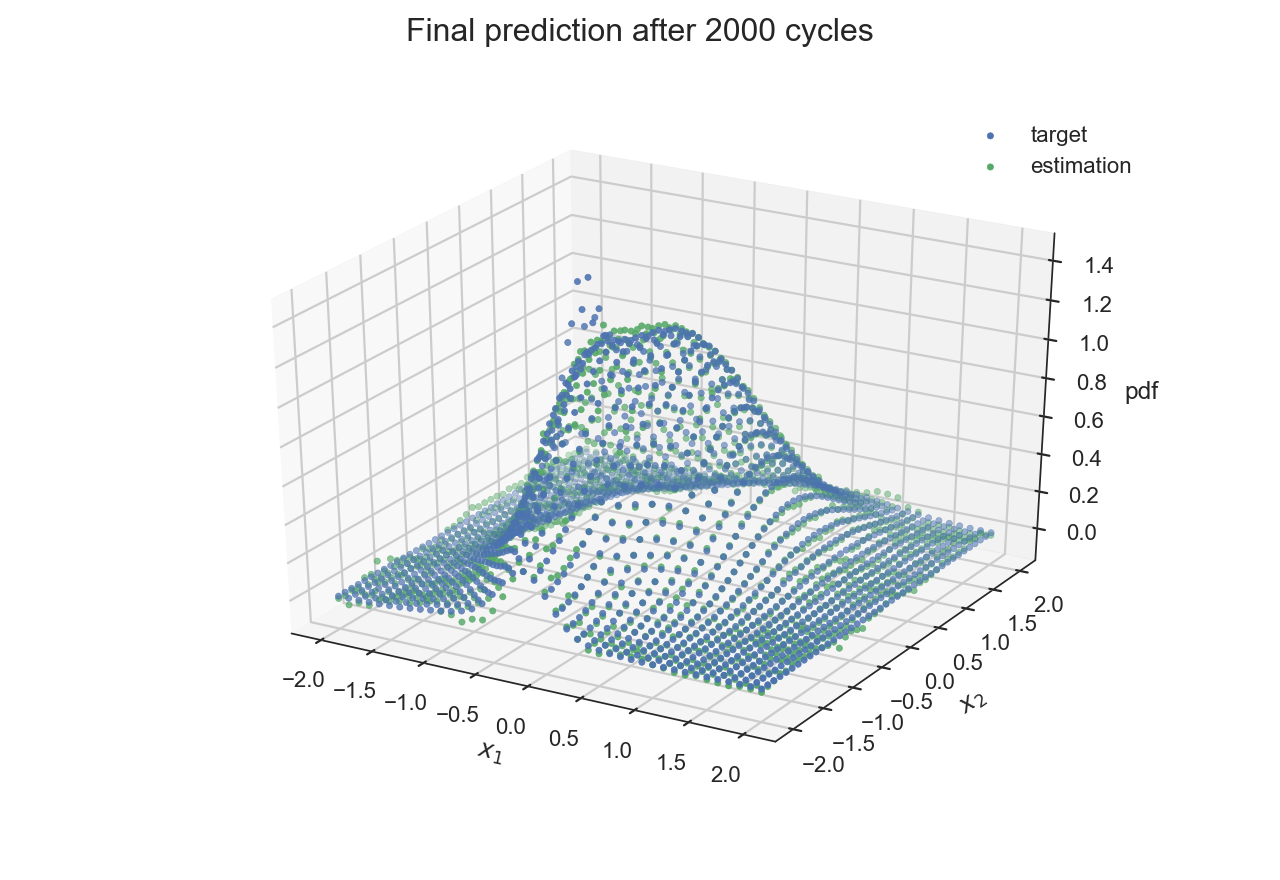
\includegraphics{../Figures/2.61}
		\caption{In green we gave the prediction generated from our network, for parameters please see the code block in this exercise. The performance of training is shown in figure \ref{fig:2.62}. Note that the little hump is not captured, but the sum squared error remains low.}
		\label{fig:2.61}
	\end{figure}

		\begin{figure}[H]
		\centering 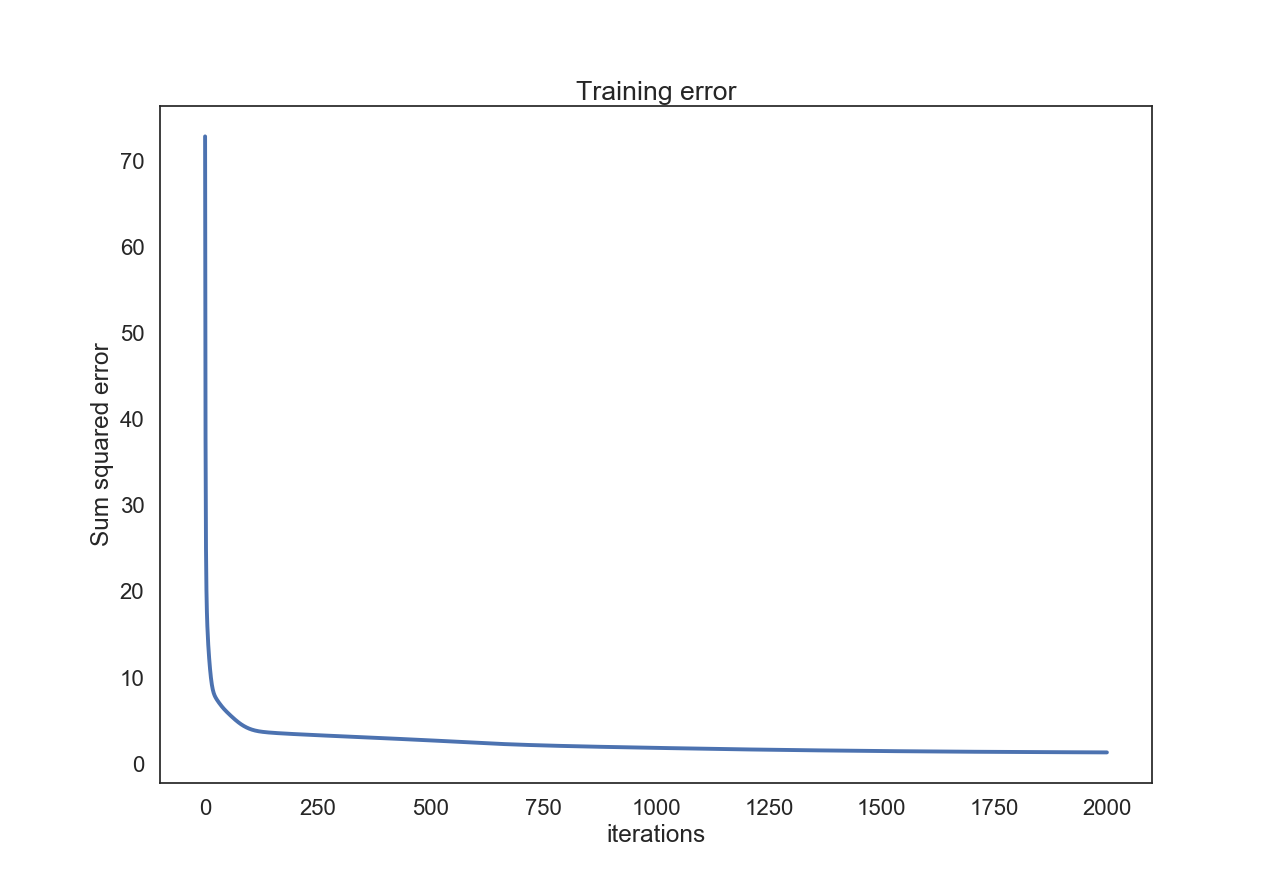
\includegraphics{../Figures/2.62}
		\caption{Sum squared error as a function of completed training cycles.}
		\label{fig:2.62}
	\end{figure}

    One might improve the performance by adding more hidden nodes to the
network. The hidden nodes essentially represent the degrees of freedom
in the model. Increasing the number of hidden nodes might increase the
fit on a trainingset, however it will also increase the modelling noise
(i.e overfitting). Improvements might also be found in presenting the
inputs / targets in a different feature space. Multi-layered perceptrons
are notorious for being sensitive to how the data is represented.
Another might be instead of taking a global learning rate, is make it
adaptive (see conjugate gradient descent, momentum etc).

    \section{7}\label{section}

    We are using python hence netlab toolbox is not available to us. We
opted for the neurolab toolbox which has a conjugate gradient method.
The same parameters were used as in 7 to improve comparison. The final output for the neurolab is represented in figure \ref{fig:2.7}. Comparisons of the training errors are displayed in figure \ref{fig:2.71}. Note, that the conjugate gradient stopped after 25 cycles, the output stated that the algorithm didn't converge. Hence, we zoomed in on the plot. The error was lower than our implementation however.

    \begin{Verbatim}[commandchars=\\\{\}]
{\color{incolor}In [{\color{incolor}101}]:} \PY{k+kn}{import} \PY{n+nn}{neurolab} \PY{k}{as} \PY{n+nn}{nl}
          \PY{k+kn}{from} \PY{n+nn}{scipy}\PY{n+nn}{.}\PY{n+nn}{optimize} \PY{k}{import} \PY{n}{fmin\PYZus{}ncg}
          \PY{c+c1}{\PYZsh{} inputs and targets}
          \PY{n}{inp} \PY{o}{=} \PY{n}{shuffX}
          \PY{n}{tar} \PY{o}{=} \PY{n}{shuffTarget}
          
          \PY{c+c1}{\PYZsh{} specify same network structure as we have}
          \PY{c+c1}{\PYZsh{} i.e. M = 40, D = 3, K = 1}
          \PY{c+c1}{\PYZsh{} this function takes min/max of input space}
          
          \PY{c+c1}{\PYZsh{} Specify activation functions;}
          \PY{c+c1}{\PYZsh{} input \PYZhy{} to hidden  is hyperbolic tangent}
          \PY{c+c1}{\PYZsh{} hidden\PYZhy{} to out is linear}
          \PY{n}{tranfs} \PY{o}{=} \PY{p}{[}\PY{n}{nl}\PY{o}{.}\PY{n}{trans}\PY{o}{.}\PY{n}{TanSig}\PY{p}{(}\PY{p}{)}\PY{p}{,} \PY{n}{nl}\PY{o}{.}\PY{n}{trans}\PY{o}{.}\PY{n}{PureLin}\PY{p}{(}\PY{p}{)}\PY{p}{]}
          \PY{n}{net} \PY{o}{=} \PY{n}{nl}\PY{o}{.}\PY{n}{net}\PY{o}{.}\PY{n}{newff}\PY{p}{(}\PYZbs{}
                             \PY{p}{[} \PY{p}{[}\PY{n}{np}\PY{o}{.}\PY{n}{min}\PY{p}{(}\PY{n}{X}\PY{p}{)}\PY{p}{,} \PY{n}{np}\PY{o}{.}\PY{n}{max}\PY{p}{(}\PY{n}{X}\PY{p}{)}\PY{p}{]} \PY{p}{]} \PY{o}{*} \PY{n}{inp}\PY{o}{.}\PY{n}{shape}\PY{p}{[}\PY{l+m+mi}{1}\PY{p}{]}\PY{p}{,}\PYZbs{}
                             \PY{p}{[}\PY{l+m+mi}{40}\PY{p}{,} \PY{l+m+mi}{1}\PY{p}{]}\PY{p}{,}\PYZbs{}
                             \PY{n}{transf}\PY{o}{=} \PY{n}{tranfs}\PY{p}{,}\PYZbs{}
                            \PY{p}{)}
          \PY{c+c1}{\PYZsh{} use conjugate gradient as method}
          \PY{n}{net}\PY{o}{.}\PY{n}{trainf} \PY{o}{=} \PY{n}{nl}\PY{o}{.}\PY{n}{train}\PY{o}{.}\PY{n}{train\PYZus{}ncg} \PY{c+c1}{\PYZsh{} conjugate gradient}
          \PY{c+c1}{\PYZsh{} net.trainf = fmin\PYZus{}ncg}
          \PY{n}{net}\PY{o}{.}\PY{n}{errorf}  \PY{o}{=} \PY{n}{nl}\PY{o}{.}\PY{n}{error}\PY{o}{.}\PY{n}{SSE}\PY{p}{(}\PY{p}{)}    \PY{c+c1}{\PYZsh{} same as above}
          
          \PY{c+c1}{\PYZsh{} init weight matrix between \PYZhy{}.5,.5}
          \PY{k}{for} \PY{n}{l} \PY{o+ow}{in} \PY{n}{net}\PY{o}{.}\PY{n}{layers}\PY{p}{:}
              \PY{n}{l}\PY{o}{.}\PY{n}{initf} \PY{o}{=} \PY{n}{nl}\PY{o}{.}\PY{n}{init}\PY{o}{.}\PY{n}{InitRand}\PY{p}{(}\PY{p}{[}\PY{o}{\PYZhy{}}\PY{o}{.}\PY{l+m+mi}{5}\PY{p}{,} \PY{o}{.}\PY{l+m+mi}{5}\PY{p}{]}\PY{p}{,} \PY{l+s+s1}{\PYZsq{}}\PY{l+s+s1}{wb}\PY{l+s+s1}{\PYZsq{}}\PY{p}{)}
          \PY{n}{net}\PY{o}{.}\PY{n}{init}\PY{p}{(}\PY{p}{)}
          
          \PY{c+c1}{\PYZsh{} Train network; show output ever 500 iterations}
          \PY{n}{errorNL} \PY{o}{=} \PY{n}{net}\PY{o}{.}\PY{n}{train}\PY{p}{(}\PY{n}{inp}\PY{p}{,} \PY{n}{tar}\PY{p}{,} \PY{n}{epochs}\PY{o}{=} \PY{n}{num}\PY{p}{,} \PY{n}{show} \PY{o}{=} \PY{l+m+mi}{500}\PY{p}{)}
          
          \PY{c+c1}{\PYZsh{} Simulate network}
          \PY{n}{outNL} \PY{o}{=} \PY{n}{net}\PY{o}{.}\PY{n}{sim}\PY{p}{(}\PY{n}{inp}\PY{p}{)}
          \PY{c+c1}{\PYZsh{} sort back to original indices}
          \PY{n}{outNL} \PY{o}{=} \PY{n}{outNL}\PY{p}{[}\PY{n}{argsort}\PY{p}{(}\PY{n}{idx}\PY{p}{)}\PY{p}{]}
\end{Verbatim}

    \begin{Verbatim}[commandchars=\\\{\}]
Warning: Warning: CG iterations didn't converge.  The Hessian is not positive definite.
         Current function value: 2.973533
         Iterations: 25
         Function evaluations: 36
         Gradient evaluations: 6893
         Hessian evaluations: 0

    \end{Verbatim}

    \begin{Verbatim}[commandchars=\\\{\}]
{\color{incolor}In [{\color{incolor}105}]:} \PY{c+c1}{\PYZsh{} plot the performance versus our algorithm}
          \PY{c+c1}{\PYZsh{} plot the final prediction and the target distribution}
          \PY{n}{fig}\PY{p}{,} \PY{n}{ax} \PY{o}{=} \PY{n}{subplots}\PY{p}{(}\PY{n}{subplot\PYZus{}kw} \PY{o}{=} \PY{p}{\PYZob{}}\PY{l+s+s1}{\PYZsq{}}\PY{l+s+s1}{projection}\PY{l+s+s1}{\PYZsq{}}\PY{p}{:} \PY{l+s+s1}{\PYZsq{}}\PY{l+s+s1}{3d}\PY{l+s+s1}{\PYZsq{}}\PY{p}{\PYZcb{}}\PY{p}{)}
          \PY{n}{ax}\PY{o}{.}\PY{n}{scatter}\PY{p}{(}\PY{n}{x}\PY{p}{,} \PY{n}{y}\PY{p}{,}\PYZbs{}
                     \PY{n}{target}\PY{o}{.}\PY{n}{reshape}\PY{p}{(}\PY{n}{x}\PY{o}{.}\PY{n}{shape}\PY{p}{)}\PY{p}{,} \PY{n}{label} \PY{o}{=} \PY{l+s+s1}{\PYZsq{}}\PY{l+s+s1}{target}\PY{l+s+s1}{\PYZsq{}}\PY{p}{)}
          \PY{n}{ax}\PY{o}{.}\PY{n}{scatter}\PY{p}{(}\PY{n}{x}\PY{p}{,} \PY{n}{y}\PY{p}{,}\PYZbs{}
                     \PY{n}{outNL}\PY{o}{.}\PY{n}{reshape}\PY{p}{(}\PY{n}{x}\PY{o}{.}\PY{n}{shape}\PY{p}{)}\PY{p}{,} \PY{n}{label} \PY{o}{=} \PY{l+s+s1}{\PYZsq{}}\PY{l+s+s1}{estimation}\PY{l+s+s1}{\PYZsq{}}\PY{p}{)}
          
          \PY{n}{ax}\PY{o}{.}\PY{n}{set\PYZus{}xlabel}\PY{p}{(}\PY{l+s+s1}{\PYZsq{}}\PY{l+s+s1}{\PYZdl{}x\PYZus{}1\PYZdl{}}\PY{l+s+s1}{\PYZsq{}}\PY{p}{,} \PY{n}{labelpad} \PY{o}{=} \PY{l+m+mi}{20}\PY{p}{)}
          \PY{n}{ax}\PY{o}{.}\PY{n}{set\PYZus{}ylabel}\PY{p}{(}\PY{l+s+s1}{\PYZsq{}}\PY{l+s+s1}{\PYZdl{}x\PYZus{}2\PYZdl{}}\PY{l+s+s1}{\PYZsq{}}\PY{p}{,} \PY{n}{labelpad} \PY{o}{=} \PY{l+m+mi}{20}\PY{p}{)}
          \PY{n}{ax}\PY{o}{.}\PY{n}{set\PYZus{}zlabel}\PY{p}{(}\PY{l+s+s1}{\PYZsq{}}\PY{l+s+s1}{pdf}\PY{l+s+s1}{\PYZsq{}}\PY{p}{,} \PY{n}{labelpad} \PY{o}{=} \PY{l+m+mi}{20}\PY{p}{)}
          \PY{n}{ax}\PY{o}{.}\PY{n}{legend}\PY{p}{(}\PY{n}{loc} \PY{o}{=} \PY{l+m+mi}{0}\PY{p}{)}
          \PY{n}{fig}\PY{o}{.}\PY{n}{suptitle}\PY{p}{(}\PY{l+s+s1}{\PYZsq{}}\PY{l+s+s1}{Neurolab prediction}\PY{l+s+s1}{\PYZsq{}}\PY{p}{)}
          \PY{n+nb}{print}\PY{p}{(}\PYZbs{}
          \PY{l+s+s1}{\PYZsq{}}\PY{l+s+s1}{final SSE neruolab :}\PY{l+s+se}{\PYZbs{}n}\PY{l+s+s1}{ }\PY{l+s+si}{\PYZob{}0\PYZcb{}}\PY{l+s+s1}{\PYZsq{}}\PYZbs{}
          \PY{o}{.}\PY{n}{format}\PY{p}{(}\PY{n}{errorNL}\PY{p}{[}\PY{o}{\PYZhy{}}\PY{l+m+mi}{1}\PY{p}{]}\PY{p}{)}\PY{p}{)}
          \PY{n+nb}{print}\PY{p}{(}\PYZbs{}
          \PY{l+s+s1}{\PYZsq{}}\PY{l+s+s1}{final SSE our alogorithm:}\PY{l+s+se}{\PYZbs{}n}\PY{l+s+si}{\PYZob{}0\PYZcb{}}\PY{l+s+s1}{\PYZsq{}}\PY{o}{.}\PY{n}{format}\PY{p}{(}\PY{n}{errors}\PY{p}{[}\PY{o}{\PYZhy{}}\PY{l+m+mi}{1}\PY{p}{]}\PY{p}{)}\PY{p}{)}
          \PY{n}{savefig}\PY{p}{(}\PY{l+s+s1}{\PYZsq{}}\PY{l+s+s1}{../Figures/2.7.png}\PY{l+s+s1}{\PYZsq{}}\PY{p}{)}
          \PY{n}{show}\PY{p}{(}\PY{p}{)}
          
          # plot training errors
          fig, ax = subplots()
          ax.plot(errorNL, label = 'conjugate gradient')
          ax.plot(errors, label = 'our MLP')
          ax.set_xlabel('Training cycles')
          ax.set_ylabel('Sum squared error')
          fig.suptitle('Conjugate gradient convergence')
          # savefig('../Figures/2.71.png')
          show()
          
\end{Verbatim}
    \begin{Verbatim}[commandchars=\\\{\}]
final SSE neruolab :
 2.9735334308131867
final SSE our alogorithm:
1.3464563919674712

    \end{Verbatim}
		\begin{figure}[H]
		\centering 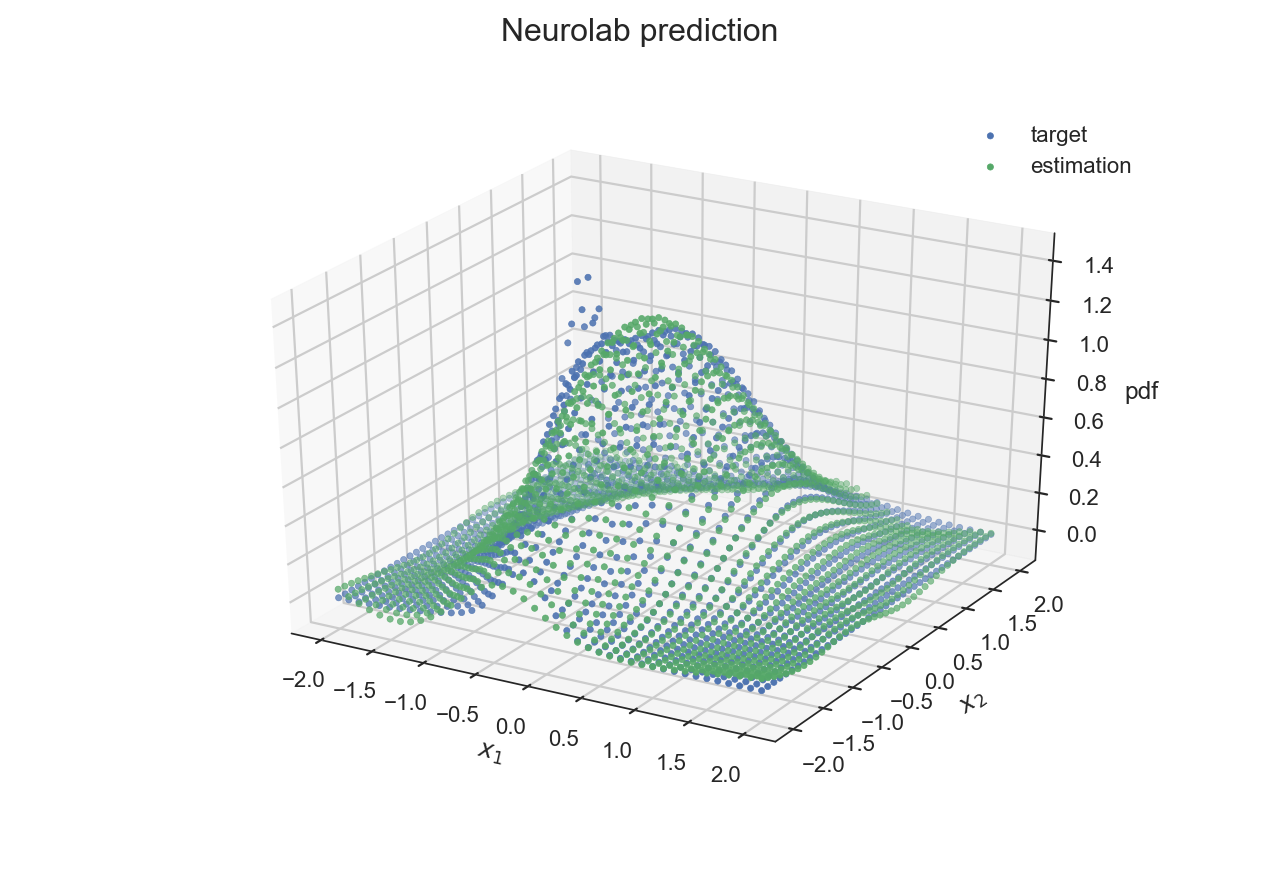
\includegraphics{../Figures/2.7.png}
		\caption{Output of conjugate gradient from neurolab toolbox.}
		\label{fig:2.7}
	\end{figure}
	
	\begin{figure}[H]
		\centering 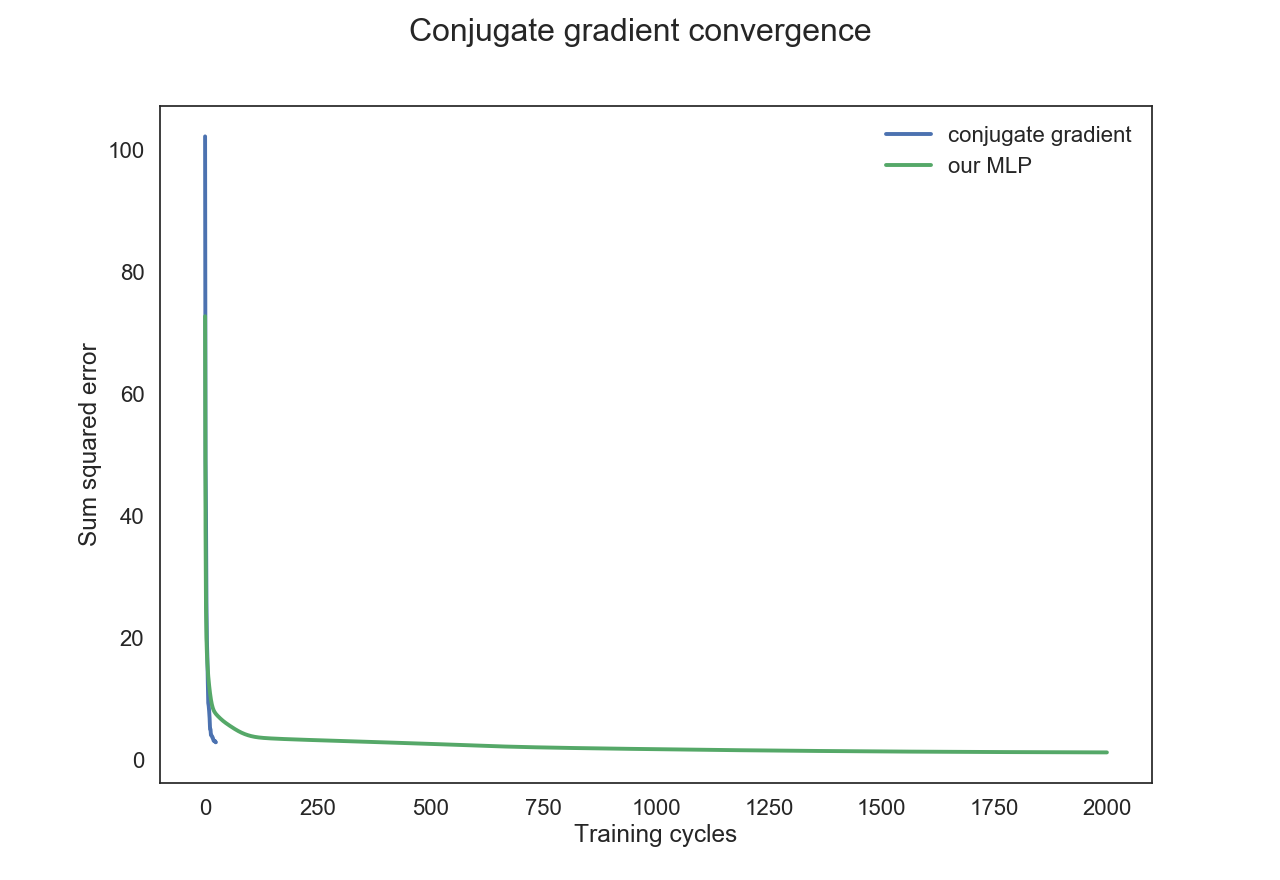
\includegraphics{../Figures/2.71.png}
		\caption{Training error of the neurolab implementation versus ours. Note that the rate of convergence if faster than our implementation. However, it did halt after 25 iterations due to a failure to converge. It uses the methods from scipy.}
		\label{fig:2.71}
	\end{figure}



    % Add a bibliography block to the postdoc
    
    
    
    \end{document}
